\documentclass[journal]{IEEEtran}
\usepackage{amsmath,amssymb,amsfonts}
\usepackage{amsthm}
\usepackage{mathtools}
\usepackage{graphicx}
\graphicspath{{figures/}}
\usepackage{booktabs}
\usepackage{array}
\usepackage[hidelinks]{hyperref}
\usepackage{url}

\newtheorem{theorem}{Theorem}
\newtheorem{lemma}{Lemma}
\newtheorem{assumption}{Assumption}
\newtheorem{definition}{Definition}
\theoremstyle{remark}
\newtheorem{remark}{Remark}

\begin{document}

\title{Harm Implies Action Deviation: A Formal Systematization of Behavioral Compromise Detection in LLM Agent Ecosystems}

\author{%
Rabie~A.~Ramadan,~Sergei~Koltcov,~Sundos~Al~Subhi,~Khalifa~M.~Al-Kindi,~and~Ahmed~Salim~Al~Rawahi%
\thanks{R.~A.~Ramadan, S.~Al~Subhi, K.~M.~Al-Kindi, and A.~S.~Al~Rawahi are with the AI Applications Chair, University of Nizwa, Nizwa 616, Sultanate of Oman (e-mail: rabie@rabieramadan.org; alkindi.k@unizwa.edu.om).}%
\thanks{S.~Koltcov is with the Laboratory for Social and Cognitive Informatics, National Research University Higher School of Economics, Sedova St. 55/2, Saint Petersburg 192148, Russia.}%
}

\markboth{IEEE Transactions on Dependable and Secure Computing}%
{Ramadan \MakeLowercase{\textit{et al.}}: Harm Implies Action Deviation}

\maketitle


\begin{abstract}
Large language model (LLM) agents now act in the world through external tools, shifting the security problem from what a model writes to what an agent does. Most deployed defenses still inspect content wehere they screen prompts, tool descriptions, and tool outputs. This is structurally limited, because the same text can be benign or harmful depending only on the action it induces, and a formal account is given of why a complementary class of defenses, which inspect behavior rather than content, is better placed. This paper has five contributions. First, a unified threat model that places the field's incompatible adversary assumptions on five axes and covers seven attack classes. Second, six behavioral compromise signatures are defined as predicates over an agent's execution trajectory. Third, if the explicit effect-through-action assumption is made, then any harmful attack, no matter where it comes from, should create an agent trajectory with an action sequence that is distinct in at least one of six ways from all benign trajectories. There is a clear distinction between definitional claims and proved results, and the completeness of the theorem is proved by an exhaustiveness lemma. Fourth, an evaluation on two public benchmarks and a controlled simulation yields a contrast with clear practical implications: behavioral detection catches nearly every attack at a near-zero false positive rate on InjecAgent (detection lower bound 0.998, false positive-rate upper bound 0.004), where attacks must invoke out-of-policy tools and sink labels are supplied by the benchmark, but achieves only 0.23 detection on AgentDojo, where attacks reuse in-policy tools, and an adaptive adversary drives simulated detection from 1.00 down to 0.79 (five-seed mean 0.79, standard deviation 0.015). Fifth, a coverage analysis that maps existing defenses to the signatures they approximate proves that detectability (unlike existence) cannot be guaranteed and uses the provable boundary to organize a research agenda. Taken together, the results connect a fragmented literature to a single question, explain rather than assert why behavioral detection generalizes across attack vectors, and locate precisely the regime in which it presently fails.
\end{abstract}

\begin{IEEEkeywords}
LLM agents, prompt injection, behavioral anomaly detection, zero trust, information flow control, AI security
\end{IEEEkeywords}

\section{Introduction}

\IEEEPARstart{F}{or} most of their short history, large language models have been used to produce text. That actually has been completely changed. An LLM agent is now understood as operating in a loop of reading its environment, deciding on an action, and then calling an external tool (typically via a standardized interface like the Model Context Protocol (MCP)) for the action, which may include a web search, a database query, a shell command, a payment API, or anything else. The model acts in ways that have effects in the world rather than only responding to a question. Files are read and written, messages are sent, and money is moved. This shift is what makes agents useful, but it also raises security concerns. It is no longer just a matter of what the model said; it is also a matter of what the agent did and which piece of input the agent believed at the time it made the decision to act.

The consequences of failing to get it right are significant. An agent can be tricked into forwarding all of a user's email to an attacker by a single sentence contained in an incoming email. An agent with access to a bank API can be directed to move the money. A user of a company's internal tools can be converted into an agent operating those same tools. None of these requires the attacker to exploit a memory corruption bug, break the encryption, or compromise the model's weights. All that is required is for the agent to read a bit of text generated by the attacker and then treat it as an instruction. What makes this difficult to defend against is the attack surface: the agent's usual activity.

The security community has responded with a growing number of defenses, but the response is far from consistent, and three structural issues plague it. Together, they form the basis of this paper; they are stated carefully here, since the remainder of the paper is devoted to solving them.

The first problem is that screening content, the dominant defensive paradigm, remains the current mainstay of deployed defense, yet it is structurally limited. All widely deployed mechanisms inspect text. A guard classifier analyzes incoming prompts and determines whether they are ``adversarial'' \cite{r1,r2}. A static checker checks the tool's description before it is registered \cite{r3} \cite{r4}. An output filter scans the output for suspicious strings. The common weakness of these mechanisms is basic rather than accidental: the same string can be completely harmless or completely catastrophic, depending solely on the agent's subsequent action.

A ``the user has asked you to delete the customer records'' tool response is merely a sentence. It is indistinguishable, as text, from a thousand benign sentences, right up until an agent treats it as an order and issues the deletion. Whether it is an attack is not a property of the text, it is a property of the action the text induces. This limitation has become a reality, not just a theory, in recent years through the work of adaptive attack researchers. When one large evaluation re-tested a dozen published prompt-injection and jailbreak defenses, most of these defenses failed against an adversary who optimized against them, rather than against the fixed, nonadaptive attacks used in the original papers, with their attack success rates moving to >90\% \cite{r5}. Attacks specifically engineered to read as natural, fluent text, including payloads generated by a tree search over phrasings, retain substantial effectiveness even when content defenses are enabled \cite{r6}. This indicates that a filtering contest cannot be won against an opponent who writes the very thing being filtered. As long as the defender's signal is the wording of the input, the attacker, who controls that wording, holds the advantage.

The second problem is quieter but no less damaging to the field's collective progress where there is no common threat model. In recent literature, different types of attack are stated.  For instance,  some attackers control the user's prompt directly \cite{r7} while others control a web page that the agent later retrieves \cite{r8}, \cite{r9}. Also, attackers may control a tool's advertised metadata, the description the agent reads to decide how to use it \cite{r10}, \cite{r11}. Moreover,  the attacker controls the live responses that a compromised tool provider streams back during the execution of a task \cite{r6}, \cite{r12}. These attacks are completely different comes from different attackers. They sit in different places in the system where they can modify different things, and their influence persists for different lengths of time such as  a single prompt is a one-shot intrusion, a poisoned tool description lasts until the tool is re-approved, a compromised provider can act on every call. Yet, the literature routinely compares defenses across these settings as though they addressed a single shared problem. Without a common set of axes on which to describe the adversary, it is impossible to say with any rigor whether a newly proposed defense closes a real gap or merely resolves, under a different name, a narrow case that earlier papers already handled. Recent surveys have done valuable work cataloging attacks and defenses \cite{r25}, \cite{r26}, but cataloging is not the same as commensurability; a list of attacks organized by descriptive category still does not indicate which defense covers which attack, or where the coverage ends.

The third problem concerns the approach identified as most promising, which is exactly what makes its present immaturity frustrating. A behavioral defense ignores the input's wording entirely and instead watches the agent. It asks operational questions about what the agent is doing: does this tool call actually serve the task the user asked for \cite{r13}; is this particular sequence of calls anomalous relative to how the task is normally accomplished \cite{r14}; is information flowing from an untrusted source into a privileged, irreversible action \cite{r15}, \cite{r16}. The appeal of this stance is that it does not depend on how the attack was delivered. A direct prompt injection, a poisoned tool description, and a corrupted tool response are three different attacks with three different delivery mechanisms, but to cause harm, all three must eventually steer the agent into doing something it should not do: that single convergence point is one place to watch instead of three. The underlying idea is not new. It is the "never trust, always verify" principle of Zero Trust Architecture \cite{r17}, a principle already applied by the security community to human insider threats through behavior analytics \cite{r18}, and applied earlier still to host intrusion through the analysis of system-call sequences and provenance graphs \cite{r21}, \cite{r27}. The difficulty is that, for agents specifically, this principle has been implemented only in fragments so far. One system enforces program-analysis constraints on the agent's runtime trace \cite{r16}, another builds an execution graph and looks for anomalies in it \cite{r14}, another models behavior hierarchically \cite{r19}, and another estimates the probabilistic reachability of unsafe states \cite{r20}. Each captures part of the idea. But they rest on incompatible assumptions, are measured on bespoke, non-comparable setups, and are almost never tested against an adversary who knows the monitor is present and is trying to evade it. There is, as a result, no shared account of how compromise actually manifests in an agent's behavior, no map connecting those behavioral manifestations back to the attacks that cause them, and almost no proof that such a manifestation must exist at all. The direction is the right one, and the evidentiary foundation beneath it is thin, both at the same time.

These three problems are not independent complaints that happen to co-occur; they are causally linked, and this link motivates the structure of this paper. Because the field lacks a common threat model (the second problem), behavioral defenses (the third problem) cannot be systematically credited for the content-level gaps (the first problem) that they are uniquely positioned to close. A behavioral defense cannot be shown to cover a class of attacks if there is no agreed-upon way to name that class of attacks in the first place. This paper provides the missing connective structure, making five contributions as follows: 

\begin{itemize}
\item A unified threat model is presented that consolidates the field's incompatible adversary assumptions into a single set of five axes (location, capability, controlled surface, persistence, and target) and shows that seven distinct attack classes correspond to seven points in that space (Section III).
\item The informal concept of ``anomalous behavior'' is formalized as six behavioral compromise signatures, defined as predicates over the execution trajectory of an agent and therefore formally checkable (Section IV).
\item A theorem of existence is proved: if an attack causes harm, it must push the agent onto a trajectory whose sequence of actions differs from every benign trajectory in at least one of these six ways, whatever injection vector was used. A distinction is maintained throughout between what follows from definitions and what requires proof, and the theorem is supported by an exhaustiveness lemma (Section IV).
\item The framework is evaluated on two public agent security benchmarks and a controlled simulation. The reported contrast is more informative than any single accuracy number: behavioral detection is near-perfect when an attack must introduce an out-of-policy tool, and weak when the attack reuses tools the agent was already permitted to call (Section V).
\item The existing defense landscape is mapped onto the signatures each defense approximates. It is proved that detectability, as opposed to mere existence, cannot be guaranteed against an adaptive adversary, and that provable boundary is used to organize a concrete research agenda (Section VI).
\end{itemize}

Section 2 positions the paper against existing surveys and prior systems, and Section VII discusses the broader implications and the path to deployment.

Therefore, this paper concerns the security of an agent's interactions with its tools and environment, the behavioral attack surface that tool use exposes. It does not concern attacks on the model's weights, such as training-time data poisoning or backdoors planted during fine-tuning \cite{r29}, nor does it concern ordinary software vulnerabilities within a tool's implementation. Those are real and important problems, but they are different problems, and they appear here only where they bear directly on the agent's observable behavior.

\section{Related Work}

The approaches proposed in related work fall into four strands (broad surveys of the agent threat landscape, content- and model-level defenses, execution- and behavior-level defenses, and the older host-security tradition of anomaly detection), and each is treated in turn, because the contribution of this paper is defined partly by how it differs from each.

The first strand is the recent wave of surveys and taxonomies that attempt to organize the agent threat landscape as a whole. He et al. \cite{r25} provide a broad treatment that organizes agent security and privacy across the planes of the engine, the instruction, the interface, the knowledge store, and the memory. Other reviews catalog the growing zoo of prompt-injection vectors and the defenses proposed against them \cite{r26}, and a more specialized line documents the security weaknesses specific to the Model Context Protocol, enumerating tool poisoning, rug pulls, and related protocol level attacks \cite{r3}, \cite{r11}. These are useful maps of the ground and form the basis for the number of attacks included here. They are not, however, equivalent to the present paper, and the difference is not merely one of magnitude. A survey is a description of attacks and defenses organized into descriptive categories. It tells what is there. It does not give a formal object in which attack is a point in an adversary space with a precise definition, nor does it (this is not possible within the survey genre) prove a relationship between attack and defense, the latter being an approximator of a predicate that can be named and checked. Although behavioral detection is found to be a promising direction, it is argued that it must work in principle, with a theorem establishing empirically where it still does not work in practice. This systematization is thus not in competition with these surveys, but rather complementary to them: they count, this paper formalizes.

The second line of defense involves content-level and model-level defenses that operate on text before it is acted upon. Input and output filtering, such as guard classifiers and programmable guardrail toolkits \cite{r1}\cite{r2}, filter the prompts that go into the model and the output that comes out of the model. Instruction-hierarchy training attempts to train the model to strengthen trusted system instructions relative to untrusted injected instructions \cite{r28}. Prompt-level isolation schemes aim to prevent untrusted data from being interpreted as instructions by the model. These are the current lines of deployed defense, and they are not worthless: they make it more expensive to carry out naive attacks. However, the literature on adaptive attacks has demonstrated repeatedly that such defenses are highly fragile when pitted against an adversary optimizing against them, rather than against a fixed benchmark \cite{r5}, and this fragility is not attributable to a lack of engineering. It stems from the structural argument introduced in the introduction; if the wording of the input is the signal of the defense, then it is playing on territory the attacker controls. The argument made here is not that these defenses should be abandoned (defense in depth has value) but that they cannot be the whole story, and the formal model in Section IV explains why.

The third strand, and the one closest to the approach developed here, comprises execution- and behavior-level defenses, which act at the moment the agent takes an action rather than at the moment it reads text. task alignment approaches check whether each tool call actually serves the user's stated task and block calls that do not \cite{r13}. Information flow control approaches track the provenance of data through the agent's execution and prevent untrusted data from reaching privileged sinks \cite{r15}, \cite{r16}. Trace and graph based anomaly detectors construct a graph that represents the execution of the agent and signal if the graph deviates from normal behavior \cite{r14,r19} and probabilistic runtime monitors estimate the probability of an execution drifting toward an unsafe state \cite{r20}. These systems represent the practical application of the behavioral approach advocated here, and Section VI relates each to the specific signatures in the taxonomy it approximates. The gap being addressed is not that these systems are wrong, but that they are fragmentary where each has its own assumptions, each is evaluated based on its own setup, and there is no proof that the behavioral signal they detect has to exist whenever an attack succeeds. The existence theorem presented here is intended to supply exactly that missing foundation, and the evaluation is intended to show, without overstatement, where even a well-constructed behavioral detector currently runs out of signal.

The fourth strand goes back even further to the host-security tradition of anomaly detection, from which the behavioral stance ultimately traces its heritage, and which affords encouragement and caution. All of these approaches to intrusion detection in systems (analyzing sequences of system calls and their arguments \cite{r21}; building event-aware program anomaly detectors for cyber-physical systems \cite{r24}; or tracing back programs to their origins via a provenance tree to detect intrusions and their real-time variants with advanced persistent threats \cite{r23,r27}) are based on the same basic intuition used in the case of agents: a compromised actor that has legitimate credentials eventually gives itself away through some form of anomalous behavior. The insider-threat literature, including LSTM-based anomaly detection for insider threats \cite{r22}, recent work that applies LLMs themselves to behavior analytics in zero-trust networks \cite{r18}, and frameworks that assess cyber-human aspects of insider threat \cite{r27}, makes the analogy to agents almost exact, a compromised agent is an insider operating with the user's own authority, distinguishable not by who it is but by what it does. This tradition also supplies a cautionary result that is relied upon heavily here. Goyal et al. showed that mimicry attacks can evade provenance graph-based host intrusion detectors by deliberately mimicking benign behavior \cite{r30}. This is treated not as a refutation of the behavioral approach but as the precise reason that existence and detectability must be kept separate in which the host-security community learned, the hard way, that a behavioral signal can provably exist and still be pushed below a usable detection threshold by an adversary who is trying to blend in. Section VI formalizes that lesson for agents.

\section{A Formal Model of Agent Compromise}

To make any of the above precise, a formal model is needed in which an agent, a task, an attack and a defense are all objects, not intuitions. In this section, that model is constructed, made as simple as possible; just the machinery needed for the theorems in the following sections. The one substantive assumption it makes is clearly mentioned and examined carefully, because the thoroughness of the entire formal structure must be apparent to the reader as to what is assumed and what is then proved.

An agent is modeled as a policy that interacts with an environment over a sequence of discrete steps. At step $i$, the agent emits an action $a_i=(t_i,x_i)$, where $t_i\in\mathcal{T}$ is the tool invoked, and $x_i$ is the arguments passed to that tool, and in response, an observation $o_i$ is received from the environment. A complete run of the agent on a task produces a trajectory, which records the full interleaving of internal states, actions, and observations:
\[
\tau = \langle s_0,\, a_1,\, o_1,\, s_1,\, a_2,\, o_2,\, s_2,\, \ldots,\, a_n,\, o_n,\, s_n \rangle.
\]
where $s_i$ denotes the agent's internal state after step $i$. $A(\tau)=\langle a_1,\ldots,a_n\rangle$ is written for the action sequence of the trajectory $\tau$, with states and observations stripped away to leave only what the agent actually did. This distinction between the full trajectory and its action sequence matters a great deal where content-level defenses inspect the text flowing through the trajectory, whereas the behavioral defenses studied in this paper inspect the shape of the action sequence itself, and the central theorem locates the evidence of compromise specifically in the action sequence rather than anywhere else in the trajectory.

A task u is the user's specification of the work the agent is intending to perform. For the purposes of this work, a task induces a structured set of expectations about what legitimate execution looks like rather than serving only as a string of instructions. Specifically, a task u induces a set of allowed tools $\mathcal{T}_u\subseteq\mathcal{T}$ that a benign execution may draw upon, an acceptable-argument set $\mathcal{X}_u(t)$ for each tool t specifying which argument values are legitimate for that tool under this task, a set $\mathcal{O}_u$ of acceptable orderings in which the actions may legitimately occur, and a set $\Pi_u$ of admissible tool selection rules, each mapping a history of prior actions to a tool that may permissibly be selected next. Admissibility of a selection is existential over this set: a tool $t_i$ is admissible after history $h_{i-1}$ when $\exists\,\pi\in\Pi_u$ with $\pi(h_{i-1})=t_i$, which makes the tool selection predicate $\varphi_2$ well-defined. The two objects are required to be consistent, in that every ordering in $\mathcal{O}_u$ is realizable by some sequence of admissible per step selections; this consistency is what the case analysis of Lemma~1 relies on when it treats orderings and selections together. Together, these four objects carve out the space of behavior consistent with correctly performing the task. The trajectories that realize this benign behavior are collected into the benign behavior set:
\begin{multline*}
\mathcal{B}(u) = \bigl\{\, \tau : \forall\, a_i=(t_i,x_i)\in A(\tau),\ t_i\in\mathcal{T}_u,\ x_i\in\mathcal{X}_u(t_i), \\
\pi(h_{i-1})=t_i \text{ for some } \pi\in\Pi_u,\ \text{and } \mathrm{ord}(A(\tau))\in\mathcal{O}_u \,\bigr\}.
\end{multline*}
It is essential to be clear about the epistemic status of $\mathcal{B}(u)$. It is a semantic object (the set of trajectories that the uncompromised agent could in fact produce while correctly executing the task), and it is not assumed to be computable, enumerable, or available to any defender. A real detector will have to approximate it from samples, and the entire difficulty of Section VI turns on the gap between the true benign set and any approximation of it. For the purposes of the theorem in Section IV, however, $\mathcal{B}(u)$ needs only to be well-defined, not computable, and it is.

With the agent, the trajectory, and the task in place, harm and, separately, attack can be defined. These are defined as distinct objects on purpose, because conflating them is exactly the error that makes existence results look tautological, and avoiding that error is one of the things this formalization is for. The discussion begins with harm, defined purely in terms of effects in the world and entirely independently of any trajectory. Let $\mathcal{E}$ be the set of external effects a run can have on the environment's privileged state (the set of consequential things that can happen, such as money being transferred or records being deleted). A harm predicate $\mathrm{Harm}:\mathcal{E}\to\{0,1\}$ designates which of these effects are harmful with respect to the task at hand. This predicate is supplied by the deployment, not derived by the agent or the defender; it encodes the policy decision about what counts as damage, and different deployments will draw the line differently. The point is that harm is a property of effects, not of trajectories or of text.

The single substantive assumption of the model, the assumption on which the central theorem depends, is now stated. It is presented as an explicit assumption so that its role is visible rather than embedded within a definition.

The effect-through-action assumption is that every effect $e\in\mathcal{E}$ that is produced by a run is caused by some action $a_i\in A(\tau)$ emitted by the agent; that is, the privileged state of the environment depends only on the agent's action output and not solely on the agent's internal reasoning. This holds for the agent architectures examined here, for a structural reason: the only way an agent can affect the world is to call tools. Stated precisely, the assumption is a closure condition on the action alphabet $\mathcal{T}$, namely that $\mathcal{T}$ enumerates every effect-producing interface available to the agent. Architectures with side channels not captured by a $(t_i, x_i)$ tuple, for example streaming partial output to a human who then acts on it, would extend $\mathcal{T}$ accordingly or fall outside the assumption's scope. The fact that reasoning results in no tool call, regardless of its malicious intent, has no external consequences whatsoever, since there is no channel through which pure deliberation can be expressed in the environment. This assumption is made explicit and given a name, rather than being embedded silently in a definition, as the entire content of the theorem relies on it. If the assumption were removed and effects were allowed to come from reasoning alone, then the theorem would not hold, and it would be correct that it does not hold, because in this hypothetical world, there would be no guarantee that compromise has any behavioral consequences whatsoever. Making this assumption explicit makes it clear that behavioral detection is possible in principle under the specified condition.

Two further definitions complete the model. The uncompromised agent is said to be bebenign, safeor a task u if no trajectory in $\mathcal{B}(u)$ produces an effect e with $\mathrm{Harm}(e)=1$, that is, if correct performance of the task never, by itself, causes harm. This is a property of the benign agent and the task, and it is the natural precondition under which the notion of "attack" is meaningful: if the uncompromised agent could cause the harmful effect on its own, then that effect cannot be attributed to any adversary. Finally, given a task u and an adversary, a run is said to be a successful attack if its trajectory $\tau'$ produces an effect e with $\mathrm{Harm}(e)=1$. What this definition does and does not say should be noted carefully. It says that a successful attack is a run that achieves a harmful effect. It does not say that the attack trajectory differs from benign trajectories: that conclusion is the work of the theorem in Section IV, and it is reached only by combining this definition with the effect-through-action assumption and benign safety. Keeping these three notions (harm over effects, safety of the benign agent, and success as the achievement of harm) formally separate is what prevents the central result from collapsing into a restatement of its own premises.

It remains to describe the adversary, and here the unification promised in the introduction takes concrete form. An adversary is described by a five tuple
\[
\mathcal{A} = (L,\, C,\, S,\, P,\, T).
\]
Whose components are each drawn from a small finite set: the location $L$ names where the adversary sits in the system; the capability $C\in\{\text{read},\text{inject},\text{modify}\}$ names what the adversary can do to the channel it controls; the controlled surface $S$ names the specific channel it manipulates; the persistence $P\in\{\text{one-shot},\text{per call},\text{cross-session}\}$ names how long its influence lasts; and the target $T\subseteq\mathcal{E}$ names the effects it is trying to bring about. Table~\ref{tab:vectors} places seven attack classes drawn from the literature into a single space, and this placement clarifies that attacks treated in the literature as though they were incomparable differ only in the values of a few well-defined coordinates. A direct prompt injection and a compromised tool provider, for instance, are not different kinds of things requiring different kinds of defense; they are the same kind of thing (an adversary injecting content) sitting at different locations with different persistence. Figure~\ref{fig:loop} shows where each adversary location attaches to the agent's execution loop, showing that the locations are not abstract categories but concrete points at which untrusted influence enters the system. The observation named in Section 1 as the field's second problem can now be stated with precision: two papers that appear to study "the same" problem are often studying different points of the adversary space, and two papers that appear to study different problems are often studying the same point. The five axes provide the vocabulary needed to distinguish which is which.

\begin{table*}[t]\centering\caption{Seven attack classes on the five adversary axes (Section~III).}\label{tab:vectors}\footnotesize\begin{tabular}{@{}llllll@{}}\toprule
\textbf{Class} & \textbf{Location} & \textbf{Cap.} & \textbf{Surface} & \textbf{Persist.} & \textbf{Target} \\
\midrule
V1 Direct inj. & User input & inject & Prompt & one-shot & Any privileged effect \\
V2 Indirect inj. & Ext. data & inject & Retrieved & per retr. & Any privileged effect \\
V3 Tool poison & Metadata & modify & Tool desc. & re-approval & Any privileged effect \\
V4 tool resp. & Tool runtime & inject & Response & per call & Any privileged effect \\
V5 Rug pull & Provider & modify & Metadata & cross-sess. & Any privileged effect \\
V6 Mem. poison & Mem. store & inject & Entries & long-term & Any privileged effect \\
V7 Inter-agent & Peer agent & inject & Messages & propagating & Any privileged effect \\
\bottomrule\end{tabular}\end{table*}

\begin{figure*}[t]\centering
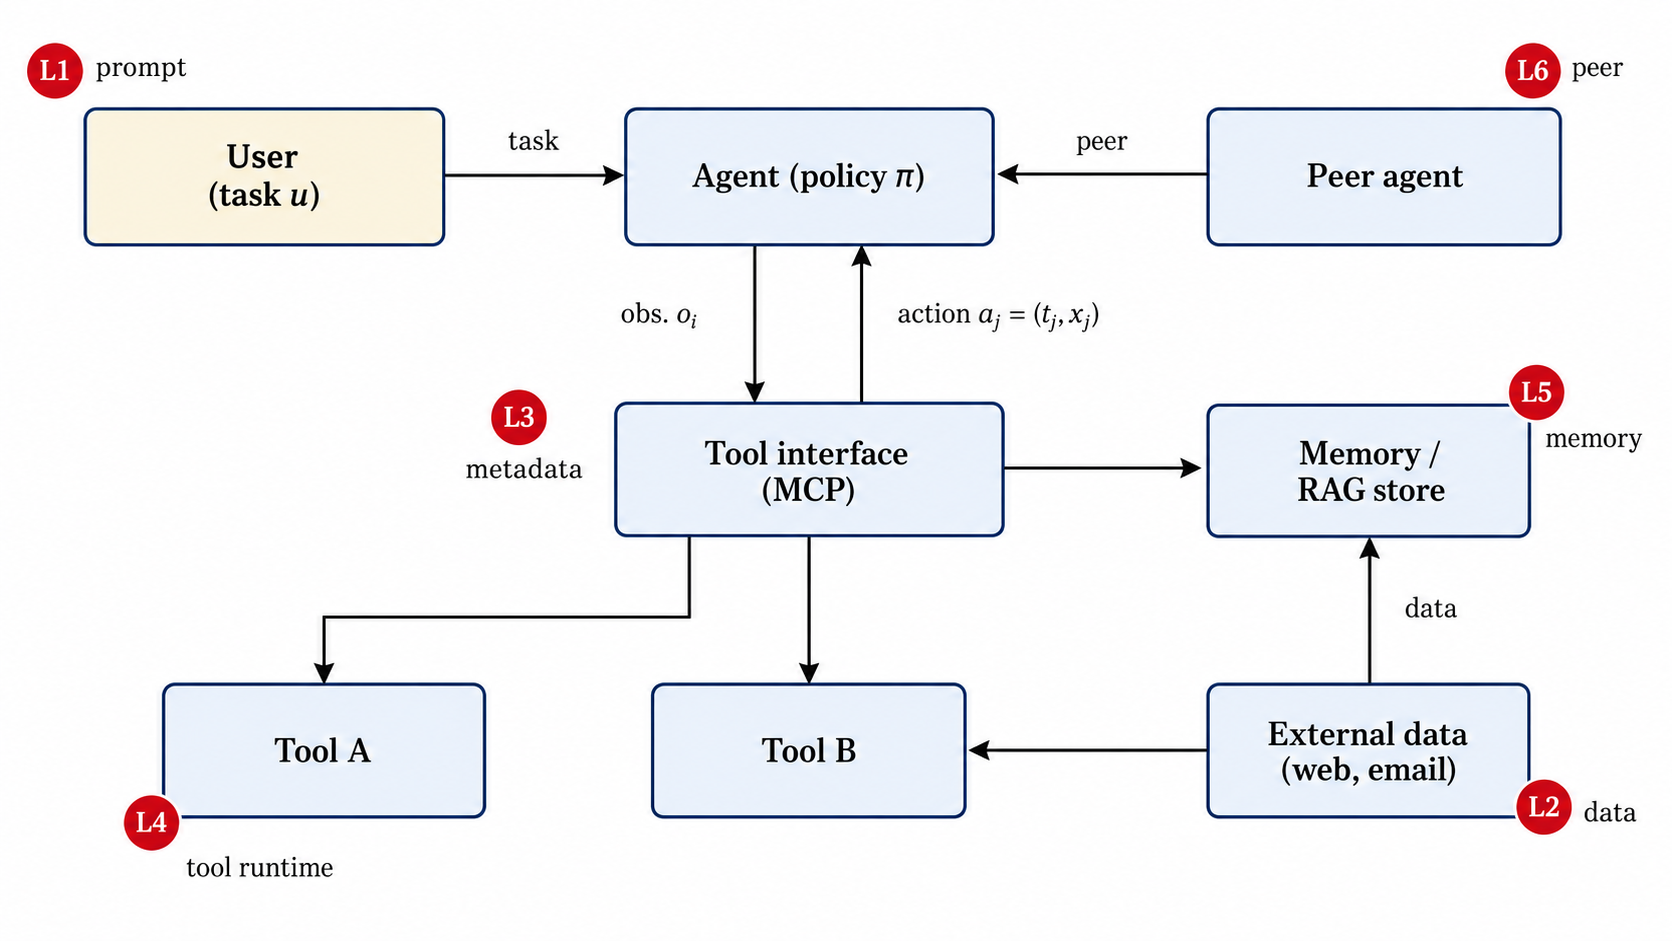
\includegraphics[width=\textwidth]{figures/fig1_agent_loop.png}
\caption{The agent loop and the six adversary locations. L1 (user prompt), L2 (external data), L3 (tool metadata), L4 (tool runtime), L5 (memory/RAG store), and L6 (peer agent) mark six of the seven Location values in Table~\ref{tab:vectors}: L1 hosts V1, L2 hosts V2, L3 hosts V3, L4 hosts V4, L5 hosts V6, and L6 hosts V7. The seventh class, V5 (rug pull), acts at the tool or model Provider, the supply-chain origin behind the tool interface, which is not drawn as a separate loop node.}\label{fig:loop}
\end{figure*}

\section{Behavioral Signatures and the Existence Theorem}

The formal model from the previous section addresses the paper's concern where the observable ways in which a compromised agent's behavior departs from benign behavior are precisely defined. It is then shown that a successful attack cannot avoid producing at least one such departure. This section constitutes the conceptual core of the paper. The six behavioral signatures are first defined as predicates over trajectories, then established as exhaustive (leaving no kind of behavioral difference uncovered), ; finally, the existence theorem itself is proved, before the whole development is grounded in a concrete worked example.

A behavioral signature is a predicate on a trajectory and a task that flags one specific kind of departure from benign behavior. Six of them are defined, and the choice of exactly these six is not arbitrary: they correspond one-to-one with the components out of which an action sequence is built, which is what makes them exhaustive. The first signature, task action divergence, fires when the agent uses a tool that lies entirely outside the set permitted for the task:
\[
\varphi_1(\tau,u) \;\Longleftrightarrow\; \exists\, a_i=(t_i,x_i)\in A(\tau) : t_i\notin\mathcal{T}_u.
\]
The second, tool selection anomaly, is subtler. It fires when the agent uses a tool that is in principle permitted for the task, but is selected in a context where no admissible selection rule would have chosen it, the right tool reached through the wrong reasoning.
\[
\varphi_2(\tau,u) \;\Longleftrightarrow\; \exists\, i : t_i\in\mathcal{T}_u \,\wedge\, \neg\,\exists\,\pi\in\Pi_u\,\bigl(\pi(h_{i-1})=t_i\bigr).
\]
where $h_{i-1}$ denotes the history of tools used before step i. The third signature, argument anomaly, fires when an action carries arguments outside the acceptable set for its tool, the right tool, permissibly selected, but handed illegitimate inputs:
\[
\varphi_3(\tau,u) \;\Longleftrightarrow\; \exists\, a_i=(t_i,x_i)\in A(\tau) : t_i\in\mathcal{T}_u \,\wedge\, x_i\notin\mathcal{X}_u(t_i).
\]
The fourth, sequence anomaly, fires when the order in which the in task actions occur violates the task's acceptable orderings. This signature is deliberately restricted to actions drawn from the allowed tool set, so that the mere insertion of an out-of-task tool (already caught by the first signature) does not also trip the fourth as a side effect, keeping the signatures independent:
\[
\varphi_4(\tau,u) \;\Longleftrightarrow\; \mathrm{ord}_{\mathrm{task}}\!\bigl(A(\tau)\bigr) \notin \mathcal{O}_u.
\]
The fifth signature, information flow violation, departs from the syntactic character of the first four and instead examines provenance. It fires when data from an untrusted source reaches a privileged sink, regardless of whether the action's surface form appears acceptable. Writing $\mathrm{Src}_\bot$ for the untrusted sources, $\mathrm{Snk}_\top$ for the privileged sinks, and $p\rightsquigarrow_\tau q$ for a data-flow path within the trajectory from p to q, the signature is defined as:
\[
\varphi_5(\tau,u) \;\Longleftrightarrow\; \exists\, p \rightsquigarrow_\tau q : p\in\mathrm{Src}_\bot \,\wedge\, q\in\mathrm{Snk}_\top.
\]
The relationship between the fifth and third signatures illustrates a subtlety where the exhaustiveness argument must be respected. An argument may be syntactically correct, such as a well-formed recipient address, even if it contains tainted data from an untrusted source. The third signature checks the value of an argument against the list of acceptable values, and the fifth signature checks the provenance of the data that flows through the action. So the fifth is not a fourth syntactic sibling, it is a semantic refinement of the third, and it is treated at the right level in the exhaustiveness proof, not presented as a partition of the same dimension. Finally, the sixth and last signature, cross-agent propagation, extends the framework to multi-agent settings. It is activated if any of the first five signatures is triggered by a message received from a compromised peer agent.
\[
\varphi_6(\tau,u) \;\Longleftrightarrow\; \mathrm{peer}(\tau) \,\wedge\, \exists\, j\in\{1,\ldots,5\} : \varphi_j(\tau,u).
\]
where $\mathrm{peer}(\tau)$ holds when the trajectory was influenced by a message from a compromised peer. The sixth signature is thus parasitic on the other five. It detects the propagation of a compromise that, in the receiving agent, must still manifest as one of the basic five departures. Table~\ref{tab:sig} summarizes the six signatures together with the practical telemetry that detecting each one requires.

\begin{table*}[t]\centering\caption{Practical interpretation of the behavioral signatures and the telemetry each requires.}\label{tab:sig}\footnotesize\begin{tabular}{@{}p{1.2cm}p{6.2cm}p{8.0cm}@{}}\toprule
\textbf{Signature} & \textbf{Practical meaning} & \textbf{Required logging} \\
\midrule
$\varphi_1$ & The agent invoked a tool that is not permitted for the current task & task identifier, invoked tool name, list of permitted tools \\[2pt]
$\varphi_2$  & The agent selected a formally permitted tool, but did so in an inadmissible context & previous tool call history, current task state, tool selection context \\[2pt]
$\varphi_3$  & The agent passed inadmissible arguments to a tool & argument values, argument schemas, admissible ranges, admissible target objects \\[2pt]
$\varphi_4$ & The agent violated the normal ordering of actions & ordered tool call sequence, admissible workflow patterns \\[2pt]
$\varphi_5$  & Data from an untrusted source reached a privileged action & data provenance, source trust labels, privileged sink labels \\[2pt]
$\varphi_6$  & Compromise was propagated through another agent & source-agent identifier, inter-agent message provenance, subsequent actions of the receiving agent \\[2pt]
\bottomrule\end{tabular}\end{table*}

This table shows that behavioral detection requires not textual analysis as such, but instrumentation of the execution trajectory. A minimal execution log must record not only the invoked tool and its arguments, but also the task, the action history, the provenance of data, and, in multi-agent settings, the source of inter-agent messages. In this sense, the proposed signatures define not only a formal taxonomy of compromise, but also a practical specification of what information a secure LLM-agent platform should collect.

With the six signatures defined, it can be established that they are collectively exhaustive where any difference between two trajectories for the same task is witnessed by at least one of them. This is the lemma on which the existence theorem will rest, and it is stated and proved carefully, since an exhaustiveness claim is only as good as its case analysis.

\begin{lemma}[Exhaustiveness]
Let $\tau$ and $\tau'$ be two trajectories for the same task $u$ with $A(\tau)\neq A(\tau')$. Their difference is witnessed by at least one of the signatures $\varphi_1$ through $\varphi_4$, and, accounting for data provenance, $\varphi_5$; in the multi-agent case, $\varphi_6$.
\end{lemma}

\begin{proof}
The proof proceeds by exhausting the ways in which two finite action sequences can differ. Two such sequences differ in exactly one of two ways. In the first case, they have different multisets of actions; some action $a_i=(t_i,x_i)$ appears in one sequence but not the other, or appears with a different multiplicity. Consider such a witnessing action. Either its tool $t_i$ lies outside the allowed set $\mathcal{T}_u$, in which case $\varphi_1$ witnesses the difference; or $t_i$ lies inside $\mathcal{T}_u$ but was selected in a context no admissible rule permits, in which case $\varphi_2$ witnesses it; or $t_i$ is admissibly selected but its arguments $x_i$ lie outside the acceptable set $\mathcal{X}_u(t_i)$, in which case $\varphi_3$ witnesses it. These three sub cases are exhaustive for a single differing action, because a tool is necessarily either disallowed, or allowed-but-misselected, or allowed-and-well-selected, and in the last sub-case only the arguments remain as a possible site of difference. A repeated in-policy action that is admissibly selected and well-argued, but that occurs a different number of times than any benign run allows, changes the ordered in task projection and is therefore witnessed by $\varphi_4$, which is read over sequences with multiplicity rather than over sets; a surplus call whose selection context is no longer admissible is instead witnessed by $\varphi_2$. The routing of a given difference between $\varphi_2$ and $\varphi_4$ is a matter of which admissibility condition it violates, and the two signatures are not claimed to have disjoint extensions; a single difference may satisfy both predicates. The lemma asserts only that at least one signature fires, so exhaustiveness is over a possibly overlapping set of predicates rather than a partition, and this weaker claim is all the existence theorem requires. In the second case, the two sequences share the same multiset of actions but differ in their order; then the ordered projection onto in task tools differs, and $\varphi_4$ witnesses the difference. A difference that is realized not in the action tuples themselves but in the data carried between them (identical actions, different provenance) is by definition a flow difference, witnessed by $\varphi_5$. A difference introduced through a message from a compromised peer reduces, in the receiving agent, to one of the previous cases and is witnessed by $\varphi_6$. The components of an action sequence, namely the tool, the selection context, the arguments, the order and multiplicity, the data provenance, and the originating agent, exhaust the ways in which two trajectories over the same action alphabet can differ, so no kind of difference escapes the six signatures, which completes the proof and the central result can now be proved.
\end{proof}

\begin{theorem}[Harm implies action deviation]
Fix a task $u$ whose uncompromised agent is benign safe and assume the effect-through-action assumption holds. If a run is a successful attack, two things follow: first, its trajectory satisfies $A(\tau')\neq A(\tau_b)$ for every benign trajectory $\tau_b\in\mathcal{B}(u)$; and second, at least one signature $\varphi_j(\tau',u)$ holds, for some $j\in\{1,\ldots,6\}$.
\end{theorem}

\begin{proof}
The proof of the first part proceeds by contradiction and is where the effect-through-action assumption does its work. By the definition of a successful attack, the run produces an effect e with $\mathrm{Harm}(e)=1$. By the effect-through-action assumption, this harmful effect is caused by some action $a_k$ in the action sequence $A(\tau')$. Suppose, toward a contradiction, that $A(\tau')=A(\tau_b)$ for some benign trajectory $\tau_b\in\mathcal{B}(u)$. Since effects are produced only through emitted actions, and $\tau_b$ shares the identical action sequence with $\tau'$, the benign trajectory $\tau_b$ produces the very same effect e. But then a benign trajectory produces a harmful effect, which contradicts the benign safety of the uncompromised agent. The supposition must therefore be false, and it is concluded that $A(\tau')\neq A(\tau_b)$ for every benign trajectory $\tau_b$. The second part now follows immediately where for any benign trajectory $\tau_b$, by the first part its action sequence differs from that of $\tau'$. So by Lemma 1 their difference is witnessed by some signature $\varphi_j$, and that witness is precisely a signature holding on the attack trajectory $\tau'$. Therefore, the proof is now completed.
\end{proof}

Two remarks fix what the theorem does and does not claim, and they matter for not overstating the result. The first concerns where the weight of the argument actually lies. It is tempting to read the theorem as stating something obvious (of course a harmful trajectory differs from benign ones), but that reading mistakes the logical structure. Harm is defined over effects, by Definition of the harm predicate, not over trajectories; nothing in the definition of harm mentions how the trajectory looks. The link from ``this trajectory caused harm'' to ``this trajectory's actions differ from every benign trajectory's actions'' is not definitional at all. It is forged entirely by the effect-through-action assumption together with benign safety, and if the effect-through-action assumption is removed (permitting harm to arise from reasoning alone), the theorem fails. That is the correct behavior for the theorem, because in such a world, nothing would guarantee a behavioral trace, and a theorem that still claimed one would be wrong. The second remark concerns where the theorem locates the deviation. It does not merely assert that the attack trajectory differs from benign ones somewhere; it locates the difference specifically in the action sequence. This is the property that makes behavioral monitoring sufficient in principle, and it is the point of contrast with content inspection. A malicious payload can be byte-for-byte identical to benign text, so content carries no guaranteed signal; but the harmful action cannot be identical, on the effect it causes, to benign behavior, so behavior does carry a guaranteed signal. The theorem is, in the end, a formal statement of why what the agent does should be watched rather than what it reads. A third remark bounds the strength of this guarantee. The theorem establishes only the existence of some signature $\varphi_j$ that fires on the attack trajectory; it does not bound the magnitude of the departure from below. The witness is guaranteed to exist, but its signal may be arbitrarily small, and Sections~5 and~6 show that an adaptive adversary can drive that margin toward zero while preserving the harmful effect. ``Sufficient in principle'' therefore means sufficient given an unbounded-precision detector, which is a strictly weaker practical claim than the existence result alone might suggest.

It helps to see the whole development on a concrete instance. Consider an email assistant whose task u is to summarize the user's latest email, so that the allowed tool set $\mathcal{T}_u$ contains \texttt{read\_inbox} and summarize, while \texttt{send\_external} is a privileged sink lying outside $\mathcal{T}_u$. A benign trajectory reads the inbox and then summarizes, and produces no external effect beyond returning a summary. Now suppose an adversary controls the body of an incoming email (the tool response injection vector, V4 in Table~\ref{tab:vectors}) and plants in it the instruction to forward all messages to an external address. If the agent is compromised by this injection, its trajectory reads the inbox, then calls \texttt{send\_external} to the attacker's address, then summarizes. This trajectory is examined against the signatures. The call to \texttt{send\_external} uses a tool outside $\mathcal{T}_u$, so $\varphi_1$ fires. Its recipient argument lies outside the acceptable set $\mathcal{X}_u$, so $\varphi_3$ fires. And untrusted content drawn from the inbox reaches a privileged external sink, so $\varphi_5$ fires. The attack arrived purely through content, a sentence in an email, but it cannot avoid surfacing in behavior, exactly as Theorem 1 requires. The mapping from injection vectors to the signatures they must produce, shown in Figure~\ref{fig:map}, is in this way derived from the theorem and the lemma rather than asserted; it is a consequence of the structure, not an assumption about it.

\begin{figure*}[t]\centering
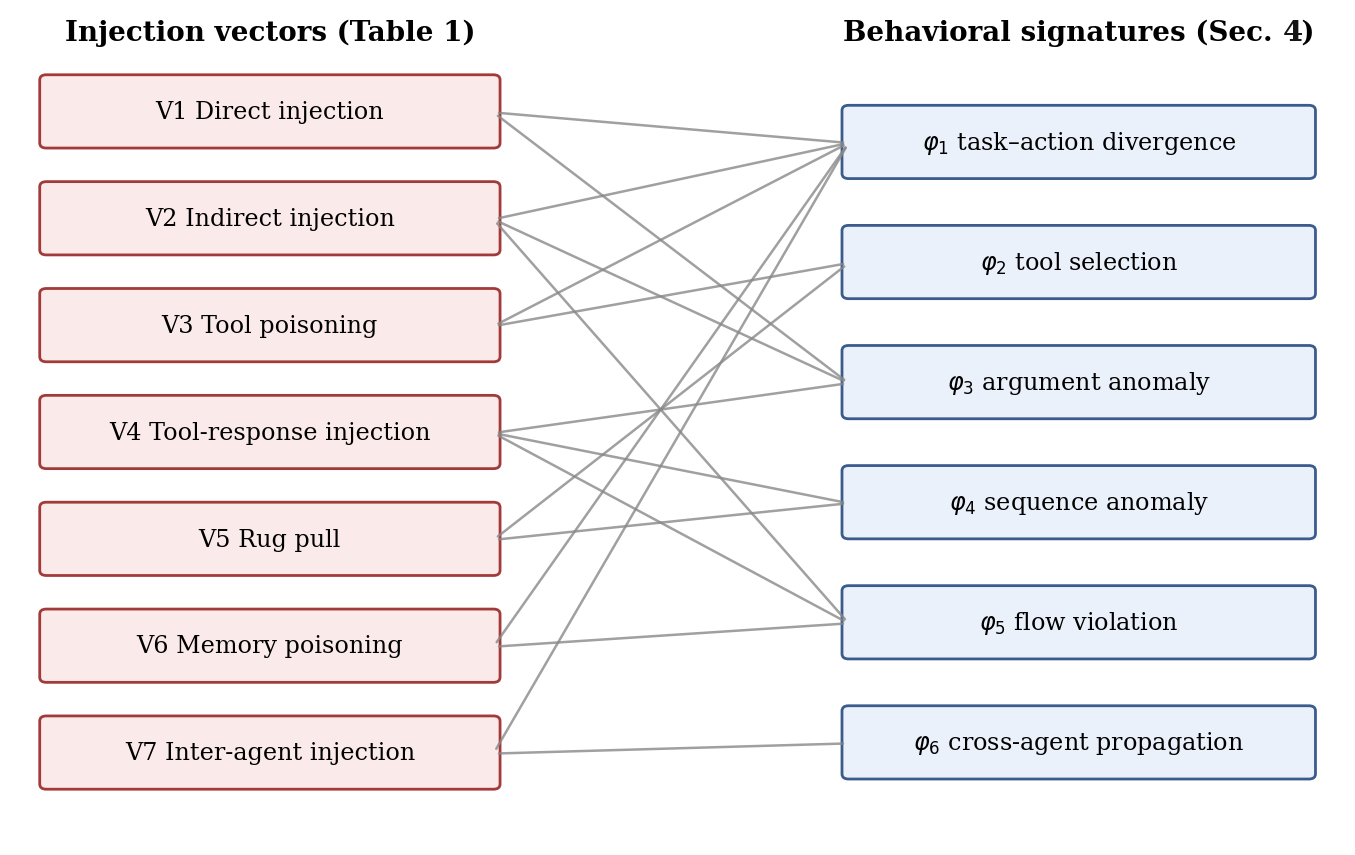
\includegraphics[width=\textwidth]{figures/fig2_vector_signature.png}
\caption{The vector-to-signature mapping, derived from Theorem 1 and Lemma 1.}\label{fig:map}
\end{figure*}

\section{Evaluation}

Theorem 1 establishes that a behavioral signature of a successful attack always exists. It says nothing, however, about whether any practical detector can find that signature once the benign behavior set must be estimated from data rather than known exactly. The gap between guaranteed existence and achievable detection is the entire engineering problem and this section measures it empirically. Evaluation is conducted in three deliberately increasing realism settings. The first is a controlled simulation, where benign behavior is generated by a known stochastic process, which allows both establishing that the detectors work when benign data is plentiful and mounting an adaptive adversary that would be prohibitively expensive on a live system. The second and third are two public agent-security benchmarks, InjecAgent and AgentDojo, run with a real tool calling agent. The headline finding is a contrast between these two benchmarks that turns out to be more informative than any single accuracy figure. Behavioral detection is near-perfect when an attack is forced to invoke a tool outside the agent's benign repertoire, and weak when the attack accomplishes its goal by reusing tools the agent was already entitled to call. The complete evaluation harness, together with the simulation generators, the calibration splits, and the scripts that regenerate every reported number, is provided as supplementary material accompanying this submission.  

\subsection{Detectors and Protocol}
Across all settings, the same detectors and protocol are used, and they are described carefully because the accuracy of the false positive numbers depends on the details. Each of the six signatures is implemented as a detector over learned normality rather than over a hand specified task specification, the allowed tools, the admissible transitions between tools, the support of acceptable argument signatures, the set of benign tool sequences, and the source and sink labels for flow are all induced from data, not supplied by an oracle. Each detector additionally produces a continuous anomaly score rather than a bare boolean, which allows calibration. The benign data is split three ways. A training portion is used to estimate the benign model. A separate calibration portion is used to select, for each signature, the score threshold at which it fires, with the threshold set to meet a target false positive rate of 5\%. A third, disjoint held out portion is used only at the very end to measure the false positive rate that is actually reported. Keeping calibration and measurement on separate data is what makes the reported false positive rate accurate rather than optimistic, because the threshold is never tuned on the data used to judge it. Two versions of the detectors are reported throughout, the calibrated detectors just described, which are the main result, and the naive exact match predicates of Section IV, which fire whenever a behavior was never seen in training and which serve as an instructive baseline. Alongside this, a content classifier is run that scans the surface text of each step for injection patterns, representing the content-inspection defense class that this paper argues is fundamentally limited. For each detector and for the ensemble, a detection rate over attack trajectories and a false positive rate over held out benign trajectories are measured. 

The overall detection rate is defined as the fraction of attacks for which at least one signature fires, and the overall false positive rate is defined as the fraction of held out benign trajectories for which any signature fires.
\[
\mathrm{DR} = \frac{\bigl|\{\tau\in\mathcal{D}_{\mathrm{atk}} : \exists\, j\; \varphi_j(\tau,u)\}\bigr|}{|\mathcal{D}_{\mathrm{atk}}|}, \qquad
\mathrm{FPR} = \frac{\bigl|\{\tau\in\mathcal{D}_{\mathrm{ben}} : \exists\, j\; \varphi_j(\tau,u)\}\bigr|}{|\mathcal{D}_{\mathrm{ben}}|}.
\]
\subsection{Controlled Simulation}
The controlled simulation establishes the framework's behavior under favorable conditions, where benign data is abundant. Four tasks are simulated (an email assistant, a web-research agent, a file manager, and a customer support agent). Each task is with its own tools, its own privileged sinks, and a stochastic benign policy that varies the length, ordering, and argument values of its trajectories from run to run, so that the benign set is diverse rather than a single repeated pattern. This yields 700 training trajectories (300 for calibration), and 600 held out for measurement, against 1680 attacks spanning all 7 vectors of the threat model. In this setting, the calibrated ensemble achieves a detection rate of 1.00 at a held out false positive rate of 0.047, exactly meeting the \(5\%\) budget. The interpretation is straightforward: when benign data is plentiful enough to estimate the benign set well, the six signatures cleanly separate attack from benign, and the calibration machinery behaves as designed. This is the framework working under controlled, favorable conditions. The benchmarks then test whether it survives contact with real agent behavior.

\subsection{Attack Generation and Reproducibility}
The simulated attacks are generated deterministically from the task specifications, without any language model in the loop, so that the harmful effect of each attack is defined by construction and benign safety holds by design. For each task, a benign skeleton is sampled from that task's weighted recipe set, and a single malicious action is inserted. The malicious action is either out-of-policy, introducing a privileged sink outside the task's allowed tool set (for example \texttt{send\_external} in the email task), or in-policy, reusing an allowed tool with an attacker-controlled argument; the harmful effect is recorded on the trajectory in both cases. Attacks are assigned round robin to the seven vectors of Table~\ref{tab:vectors}, with the cross-agent vector marking the trajectory as peer-compromised. At the default settings this produces 700 training, 300 calibration, and 600 held out benign trajectories against 1680 attacks (420 per task, four tasks). The adaptive adversary applies a cumulative, monotone, effect preserving perturbation ladder to each successful attack where budget one relocates the malicious action to a high-frequency benign position, budget two surrounds it with its most common benign predecessor, budget four launders the provenance label from untrusted to trusted, and budget eight reroutes the action to an allowed tool carrying benign looking arguments. Every level preserves the recorded effect and only alters the observable surface; therefore, higher budget never increases detectability.

Because both the benign policy and the adversary are stochastic, every reported simulation figure is the mean over five random seeds, reported with its standard deviation, following the variance-aware benchmarking protocol of \cite{r31}. The seeds are fixed in advance and every run is reported. This protocol is what surfaced the seed sensitivity of the real data adaptive collapse discussed below.

\subsection{Benchmark Results: The Central Contrast}
The two benchmarks yield the paper's central result, presented as a contrast. Table~\ref{tab:detect} and Figure~\ref{fig:detfp} lay out the headline numbers across all three settings. 
On InjecAgent, evaluated across its four variants comprising roughly 2,100 attacks and roughly 1,000 held out benign trajectories, the calibrated ensemble detects every single attack at a false positive rate of zero, far above the content baseline, which achieves only about 7\% detection on the base variants. On AgentDojo, the same ensemble (same detectors, same protocol) achieves a detection rate of only 0.23, while the naive exact-match detectors fire on fully  88\%  percent of benign runs. Taken at face value, these two outcomes appear contradictory where the same method cannot readily be both near perfect and nearly useless. The resolution lies in examining which signatures actually fire in each case, shown per signature in Figure~\ref{fig:persig}. On InjecAgent the detection is carried by the task -action-divergence, tool selection, and information flow signatures, all three at a detection rate of 1.00. Every InjecAgent attack works by inducing the agent to invoke an attacker tool that no benign run for that task ever uses. The compromise steps outside the benign tool repertoire, which is exactly what these signatures are built to catch. The attack cannot help but be visible, because it cannot accomplish its goal without calling a tool that flags. On AgentDojo the situation is reversed. There, the attacker does not introduce a new tool at all; it coerces the agent into misusing tools it was already permitted to call, sending money through the legitimate transfer tool, for instance, merely to the wrong recipient. The out-of-policy signatures, therefore, have almost nothing to flag, because no out-of-policy tool ever appears, and detection falls back onto the weaker sequence and argument signals, which, on this small and diverse benign sample, cannot establish a stable enough notion of normal to separate attack from benign. All detection and false positive rates in this section carry exact Clopper  Pearson 95\% confidence intervals: on InjecAgent the detection rate of 1.00 ($\approx$2,100 attacks) has a lower bound of 0.998 and the zero false positive rate ($\approx$1,000 benign) an upper bound of 0.004, and the controlled-simulation detection rate of 1.00 (1,680 attacks) has a lower bound of 0.998; confidence intervals for the reconstructed AgentDojo trajectories are reported in the ground truth analysis below.

This contrast constitutes the paper's empirical thesis, stated plainly as behavioral detection is strong exactly when an attack is forced to introduce out-of-policy behavior, and weak when the attack stays within the agent's existing policy. The boundary between the easy and hard regimes is not a matter of detector tuning that more engineering would fix; it is a property of the attack itself, of whether accomplishing the adversary's goal requires stepping outside what the agent was already allowed to do. This reframes the open problem in the field. The question is not "does behavioral detection work" (it provably does, in the sense of Theorem 1, and it empirically does in the out-of-policy regime) but rather "can behavioral detection be made to work in the in-policy regime," where the signal is faint because the attack hides among legitimate uses of legitimate tools.

\subsection{Why in-policy Attacks Are the Hard Case}
This contrast identifies the in-policy regime as the hard case. The difficulty of detection depends on detector quality and also on whether the adversary must leave the task's permitted action space in order to cause harm. In the out-of-policy regime, the adversary must induce the agent to perform an action that clearly falls outside the behavior permitted for the task. Such a deviation typically appears as a forbidden tool call, an information flow violation, or an obvious departure from an admissible trajectory. This is why the signatures $\varphi_1$, task action divergence, and $\varphi_5$, information flow violation, are especially strong in that regime.

The situation is different in the in-policy regime. Here, the adversary does not introduce a new tool and does not necessarily violate the coarse structure of the workflow. Instead, the agent is caused to misuse a tool that already belongs to the admissible action set. In this case, harm arises not from the mere fact that the tool is invoked, but from a wrong recipient, wrong object, wrong amount, wrong timing, wrong justification, or untrusted data provenance.

Consider a financial agent whose user task is stated as:

\[
u=\text{``pay my electricity bill''}
\]

For this task, the funds transfer tool may be admissible:

\[
\texttt{transfer\_funds}\in \mathcal{T}_u
\]

A benign trajectory may include reading the invoice, verifying the payee, and calling

\[
\texttt{transfer\_funds}(\mathit{amount},\mathit{recipient})
\]

If an adversary substitutes the payment details in the invoice, the agent may invoke the same admissible tool in the same broad sequence of actions, but with an incorrect value of the recipient argument. In this case, the task -action divergence signature does not fire:

\[
\varphi_1(\tau,u)=0
\]

Because the tool remains admissible, the action sequence may also appear admissible, so $\varphi_4$($\tau$,u) may not provide a reliable signal. Detection must therefore rely on finer grained evidence: an argument anomaly, $\varphi_3$($\tau$,u), if the recipient does not belong to the acceptable set of values, or an information flow violation, $\varphi_5$($\tau$,u), if the recipient details originate from an untrusted source and are then used in a privileged action.

Thus, in-policy attacks are difficult not because a behavioral trace is lacking. By Theorem 1, such a trace must exist. They are difficult because the trace has a small observable margin: the harmful action is disguised as a legitimate use of a legitimate tool. In this regime, the practical task of the detector is not to identify a forbidden tool, but to determine whether a particular use of an admissible tool is consistent with the user's intent, acceptable arguments, and trusted data provenance.

\subsection{ground Truth Reconstruction of AgentDojo: Provenance as the Lever}

To probe the in-policy regime directly, and to fix the denominators the live runs leave implicit, the AgentDojo trajectories are reconstructed from the benchmark's ground truth annotations, which specify for every user task and every injection task the canonical sequence of tool calls. This yields 97 benign trajectories and 629 attack trajectories (the full user-task by injection-task grid), deterministically and without executing any language model. These 97 reconstructed benign trajectories are distinct from the 65 benign trajectories collected from live AgentDojo runs used for calibration in the preceding subsections: the 65 back the 0.23 live-detection figure, whereas the 97 canonical reconstructions back the provenance ablation figures (0.151 and 0.968) reported here.

On these trajectories, detection is found to depend almost entirely on whether provenance (taint) labels are available. When restricted to the argument and sequence signatures (the signals obtainable without provenance), the calibrated ensemble detects 0.151 of attacks (95\% CI [0.124, 0.181]). Adding the information flow signature $\varphi_5$, which requires provenance labels on tool outputs, raises detection to 0.968 (95\% CI [0.951, 0.980]). The no provenance figure brackets the 0.23 obtained on the live AgentDojo runs; the residual gap reflects the thinness of the benign calibration sample (only 97 benign trajectories exist), which is itself one of the detectability limits formalized in Section VI.

The lesson exceeds what any single number can convey. in-policy attacks reuse admissible tools with plausible arguments, so task action divergence cannot fire; whether they are detectable at all hinges on the integrity of provenance tracking. Reliable taint propagation is therefore identified as the most valuable input for detecting in-policy compromise, converting a near-invisible 0.15 into a highly detectable 0.97 (Fig.~\ref{fig:gt}). Obtaining such labels in practice is itself an open problem: MCP servers are frequently Third party and closed-box, exposing no taint-propagation hooks, so provenance must be reconstructed at the host layer by tracking which upstream content influenced which downstream call, a dynamic-taint problem made harder by the non-deterministic, LLM-mediated data flow between tools. The lever this paper identifies is thus the most valuable input and, at present, among the hardest to supply.

\begin{figure}[t]\centering
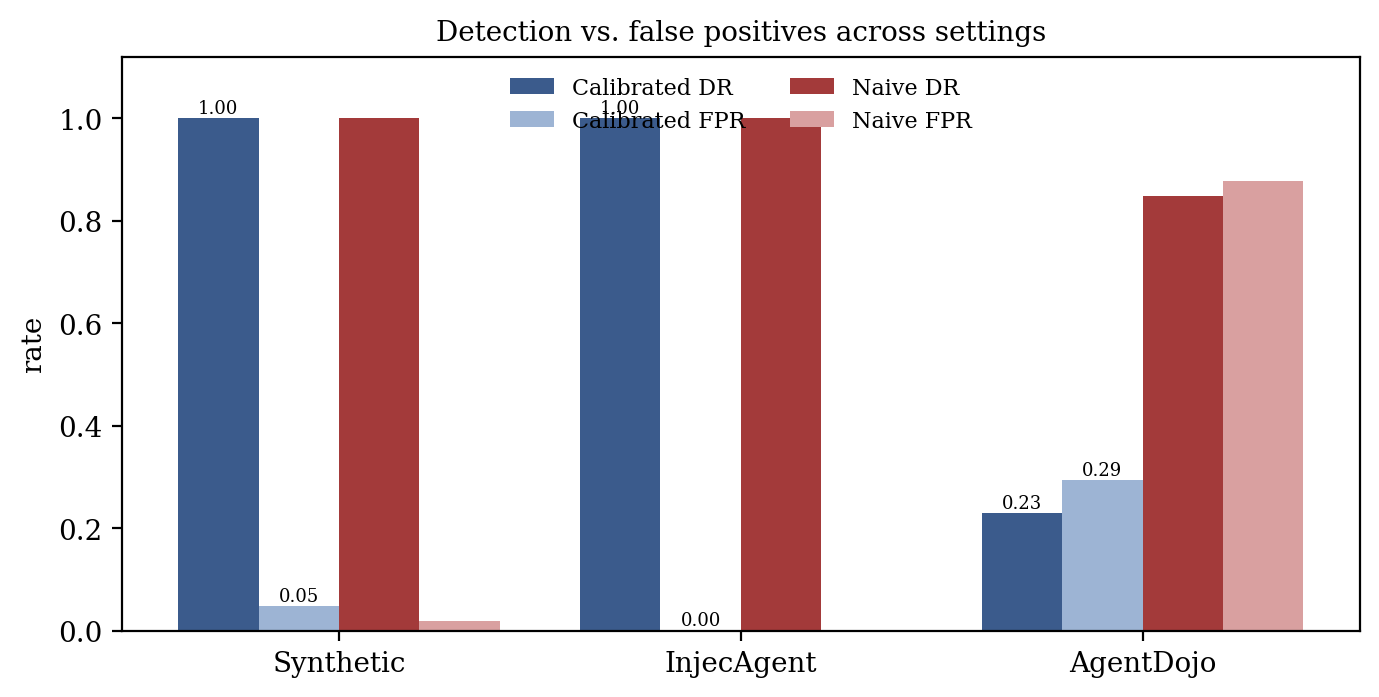
\includegraphics[width=\columnwidth]{figures/fig3_detection_fp.png}
\caption{Detection and false positive rates across settings.}\label{fig:detfp}
\end{figure}

A balanced account requires equal clarity about the factors that flatter and that penalize these numbers, and there are two of each. On the flattering side, InjecAgent's privileged sinks are taken directly from the benchmark's own labeling of which tools are attacker tools, rather than being independently inferred, which makes the fifth signature's job easier than it would be in a deployment where sink labels must be discovered; and the content baseline degenerates on the ``enhanced'' InjecAgent variants, firing indiscriminately on every run because the injected text appears in every tool response there, benign and attacked alike, so the baseline is reported only on the base variants where it remains meaningful. On the penalizing side, AgentDojo offers only 65 benign training trajectories spread across four very different task suites, which is far too few to estimate the benign behavior set well, and that scarcity is part of why calibration cannot recover detection in the hard regime; and only the indirect, tool response injection vector is exercised by the live benchmarks, so the remaining six vectors of the threat model are evaluated only in simulation. A direct symptom of this scarcity is that the calibration does not transfer on AgentDojo: thresholds selected for a five percent false positive target on the calibration split yield a held out false positive rate of 0.29, because the estimated benign set is too incomplete for any single threshold to hold the target while retaining detection. None of these caveats overturned the central contrast (the easy and hard regimes are separated by the structure of the attack, not by these measurement artifacts), but stating them is necessary for the numbers to be trusted in the direction they point.

\subsection{Attack Classes and the Value of a Second Live Vector}
The detectability-relevant distinction is not between benchmarks but between attack classes, out-of-policy attacks, which must invoke a tool no benign run for the task ever uses, and in-policy attacks, which misuse an already-admissible tool. InjecAgent is out-of-policy and is detected near-perfectly; AgentDojo is in-policy and is the hard case. Agent Security Bench \cite{r10} was examined as a candidate second live vector for its tool poisoning attacks, in which poisoned tool descriptions lure the agent into calling an attacker tool. In that benchmark's released data every attacker tool lies outside its agent's normal tool repertoire, so tool poisoning is structurally out-of-policy (the same class as InjecAgent), and it is detected by the framework through the same task action-divergence and tool selection signatures. A second out-of-policy benchmark therefore corroborates the easy regime rather than stressing the hard one; the discriminating evaluation remains the in-policy regime, which is why the analysis is concentrated there. An adapter that maps Agent Security Bench runs onto the trajectory representation is provided with the released code so this vector can be measured directly on any deployed model.

\begin{table}[t]\centering\caption{Calibrated vs.\ naive detection across settings, with content baseline. $^{*}$Baseline meaningful only on InjecAgent base variants.}\label{tab:detect}\footnotesize\begin{tabular}{@{}lccccc@{}}\toprule
\textbf{Setting} & \textbf{C-DR} & \textbf{C-FPR} & \textbf{N-DR} & \textbf{N-FPR} & \textbf{Base} \\
\midrule
Simulation & 1.00 & 0.05 & 1.00 & 0.02 & 0.86 \\
InjecAgent & 1.00 & 0.00 & 1.00 & 0.00 & 0.07* \\
AgentDojo & 0.23 & 0.29 & 0.85 & 0.88 & 0.25 \\
\bottomrule\end{tabular}\end{table}

\begin{figure}[t]\centering
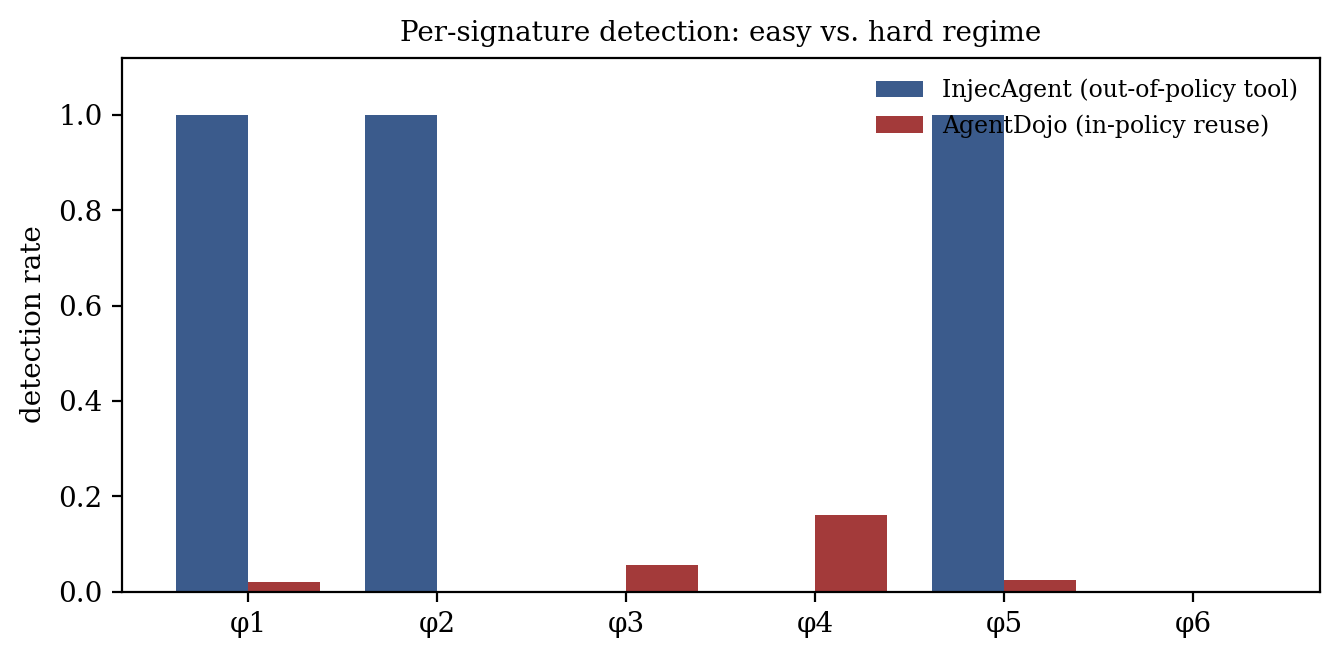
\includegraphics[width=\columnwidth]{figures/fig4_per_signature.png}
\caption{Per signature calibrated detection: phi1/phi5 carry InjecAgent; AgentDojo has little to flag.}\label{fig:persig}
\end{figure}

\begin{figure}[t]\centering
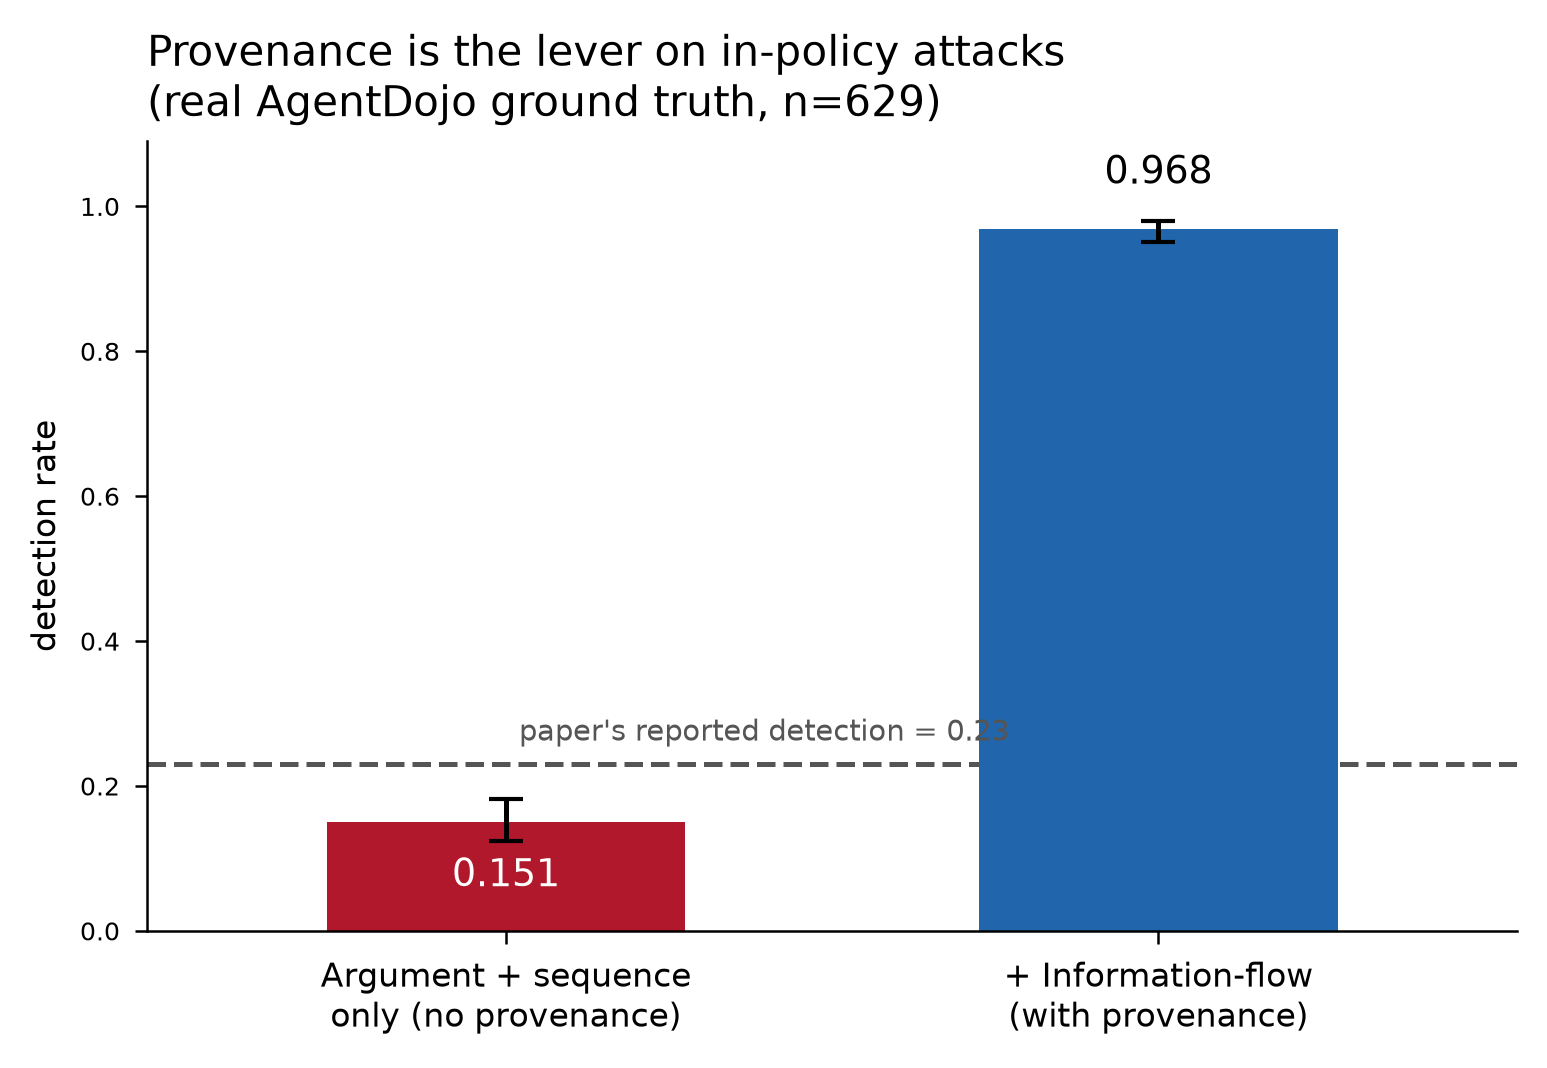
\includegraphics[width=\columnwidth]{figures/fig6_inpolicy_groundtruth.png}
\caption{in-policy detection on 629 ground truth AgentDojo attack trajectories, with and without the provenance dependent information flow signature. Error bars are exact 95\% confidence intervals; the dashed line marks the 0.23 obtained on the live runs.}\label{fig:gt}
\end{figure}

\subsection{Adaptive Adversary}
The adaptive adversary is evaluated in the simulation, where attacks can be perturbed freely while their harmful effects are preserved, which would be difficult to guarantee in a live benchmark. Starting from each successful attack, effect-preserving perturbations of increasing budget are applied: at low budget the malicious action is relocated to a high-frequency position and its arguments are renamed to trusted-looking values; at higher budget an out-of-task tool is replaced with an allowed tool carrying the same effect; and at the highest budget the malicious effect is embedded inside a sampled benign skeleton with its provenance laundered, reconstructing an attack that mimics a benign trajectory as closely as the effect allows. Table~\ref{tab:adaptive} and Figure~\ref{fig:adsim} show the results, and their shapes are faithful measures of the approach. Detection remains flat and near-perfect at low budget (1.00 through budget four) and then falls to 0.79 at the highest budget (five-seed mean 0.788, standard deviation 0.015; each figure is the mean over five random seeds, reported with its standard deviation). The interpretation aligns exactly with the theory of Section VI: Theorem 1 continues to hold for every budget, so a signature always exists, but a determined adversary who reconstructs a near-benign trajectory can push the witnessing signal below the detector's threshold. A flat curve here would have been a warning sign, evidence of an adversary too weak to take seriously rather than a defense strong enough to trust; the collapse is the expected and correct behavior, and it is the empirical face of the existence versus detectability gap that the next section formalizes. The evaluation concludes by noting that the signature-scoring overhead is negligible (on the order of three microseconds per action in this implementation), measured as the cost of evaluating the six predicates over features already collected. This figure excludes the cost of collecting those features, in particular the provenance labels that $\varphi_5$ requires: taint propagation across tool calls, which in an MCP topology of Third party servers is the expensive and, as Section~6 discusses, not always available component. The scoring step is therefore cheap, but the instrumentation that supplies its inputs is not uniformly so, and the two costs are reported separately for this reason.

The adaptive adversary analysis extends directly to the real AgentDojo benchmark data. When a cumulative, effect-preserving perturbation ladder is applied to the reconstructed AgentDojo attack trajectories (relocating the injected call, laundering cosmetic arguments to benign values, forging provenance labels, and padding with a benign predecessor, while always preserving the injected call that carries the harmful effect), detection holds at 0.97 through the first two budget levels (five-seed mean 0.969, standard deviation 0.002), then falls once the adversary forges provenance: to a five-seed mean of 0.55 (standard deviation 0.24) at budget four and 0.11 (standard deviation 0.13) at the highest budget (Fig.~\ref{fig:adreal}). The large standard deviation at the two highest budgets is itself a finding: the collapse is real but seed-dependent, ranging across seeds at budget four from a near-total collapse (0.36) to almost no collapse at all (0.97), so the collapse is best characterized by its five-seed distribution rather than by any single-seed curve. The collapse still localizes at provenance laundering. This confirms on real data both the adaptive degradation thesis and the diagnosis above: detection of in-policy attacks is load-bearing on the information flow signature, so an adversary able to forge trust labels defeats it. Provenance integrity is thus simultaneously the strongest lever for the defender and the single point of failure an adaptive attacker will target.

The budget ladder can be priced in dollars to make the adversary's effort concrete. Each rung is one incremental operation; two rungs (relocating the malicious call and forging the provenance label) are bookkeeping edits that call no model, while the other two (laundering cosmetic arguments and rerouting to an allowed tool) require a single rewrite call. Priced against GPT-4o list rates (\$2.50 per million input tokens and \$10.00 per million output tokens, the model used by the InjecAgent and Task Shield references), reaching the provenance forging rung costs on the order of a quarter of one US cent per attack, and the full ladder costs under one cent (Fig.~\ref{fig:addollar}). The decisive observation is that detection on AgentDojo falls vertically on this cost axis: the provenance forging rung, which triggers the collapse, adds no dollar cost because it makes no model call. The adaptive collapse is therefore not bought with a larger compute budget but with the ability to write a trust label, which is free. A cost model does not soften the vulnerability; it shows that the single point of failure is also the cheapest one to attack.

\begin{figure}[t]\centering
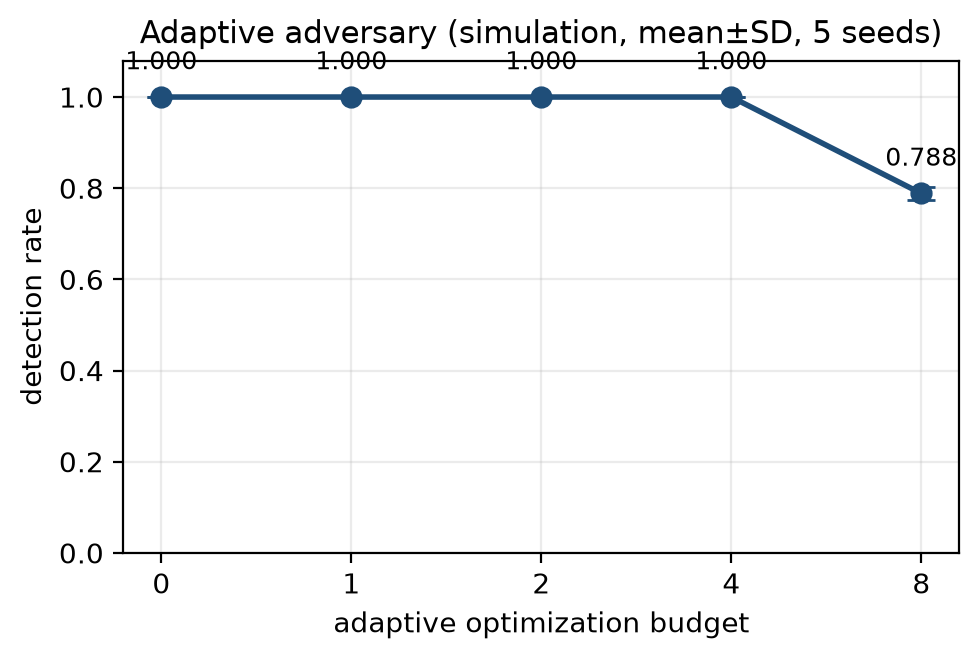
\includegraphics[width=\columnwidth]{figures/fig5_adaptive_sim.png}
\caption{Detection under an adaptive adversary (simulation), mean over five-seeds with one-standard-deviation error bars.}\label{fig:adsim}
\end{figure}

\subsection{Comparison with provenance Aware Defenses}
A natural question is whether the lift from 0.151 to 0.968 is specific to these six signatures or generic to any detector that reads provenance. To answer it, three published behavioral defenses were run on the identical 629 attack trajectories and held out benign set: a task alignment check in the style of Task Shield \cite{r13}, a taint-typing check in the style of AgentArmor \cite{r16}, and a planner/executor information flow check in the style of f-secure IFC \cite{r15}. Each was given the side information its published mechanism requires. Table~\ref{tab:baselines} reports the outcome.

\begin{table}[t]\centering\caption{adaptive adversary degradation in simulation. Each detection rate is the mean over five random seeds; the standard deviation is shown below it ($n=1680$ attacks per seed).}\label{tab:adaptive}\footnotesize\begin{tabular}{@{}lccccc@{}}\toprule
Budget & 0 & 1 & 2 & 4 & 8 \\
\midrule
Detection (mean) & 1.00 & 1.00 & 1.00 & 1.00 & 0.79 \\
Std.\ dev. & 0.00 & 0.00 & 0.00 & 0.00 & 0.015 \\
\bottomrule\end{tabular}\end{table}

The comparison is deliberately not framed as a claim of superiority. Every provenance aware detector, ours included, recovers the in-policy attacks at essentially the same rate (0.968), which makes the underlying point precise: provenance, not any particular signature set, is what makes in-policy detection possible. The distinction the six signatures offer is what they do \emph{not} require. The task alignment and taint-typing detectors need a clean task specification or explicit sink labels to reach their numbers, whereas the signature ensemble estimates normality from benign trajectories alone and needs only provenance labels, which are the one input all effective detectors here share. The contribution is therefore best read as spec free behavioral detection that matches spec based enforcement once provenance is available, and the appropriate takeaway is the shared dependency: absent trustworthy provenance, none of these defenses detect the in-policy attack.

For completeness, the numbers each system reports on its own benchmark are noted here as published context rather than as directly comparable rows. AgentArmor reports a detection rate of 0.93 at a false positive rate of 0.02 on AgentDojo under GPT-4o~\cite{r16}; Task Shield reduces attack success to 2.07\% while holding utility at 69.79\% on AgentDojo~\cite{r13}; and the information flow system drives InjecAgent attack success to 0\%~\cite{r15}. These figures come from each system's own setup and metric (attack success rate for the two enforcement defenses, which do not report a detection-rate and false positive pair), so they are not placed in the table above, which reports every detector on the identical 629-trajectory reconstruction. The proxy rows are faithful reimplementations of each published decision rule and give the same-data comparison the reported numbers cannot.

\begin{figure}[t]\centering
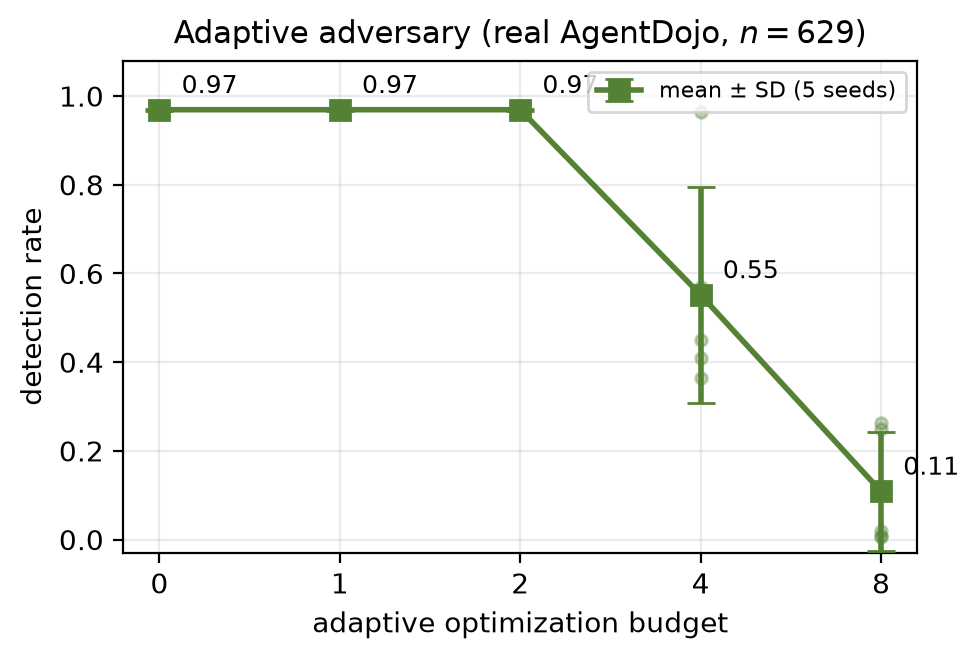
\includegraphics[width=\columnwidth]{figures/fig7_adaptive_real.png}
\caption{Detection under a monotone, effect-preserving adaptive adversary on the 629 real AgentDojo attack trajectories, averaged over five random seeds (markers show individual seeds; error bars show one standard deviation). Detection falls once provenance is laundered at budget 4; the wide spread at budgets 4 and 8 shows the collapse is real but seed-dependent.}\label{fig:adreal}
\end{figure}

\begin{table}[t]\centering\caption{Competing behavioral defenses on the 629 ground truth AgentDojo attacks (same held out benign split). Each row lists the side information the mechanism consumes. Implementations are faithful proxies of each published decision rule.}\label{tab:baselines}\footnotesize\begin{tabular}{@{}lccp{2.5cm}@{}}\toprule
\textbf{Detector} & \textbf{DR} & \textbf{FPR} & \textbf{Side information} \\
\midrule
Ours, $\varphi_1$--$\varphi_4$ (no provenance) & 0.151 & 0.04 & none (learned from benign) \\
Ours, $\varphi_1$--$\varphi_6$ (with provenance) & 0.968 & 0.04 & provenance labels \\
Task Shield proxy \cite{r13} & 0.955 & 0.00 & task specification \\
AgentArmor proxy \cite{r16} & 0.968 & 0.00 & provenance labels \\
f-secure IFC proxy \cite{r15} & 0.968 & 0.00 & provenance + plan \\
\bottomrule\end{tabular}\end{table}

\begin{figure}[t]\centering
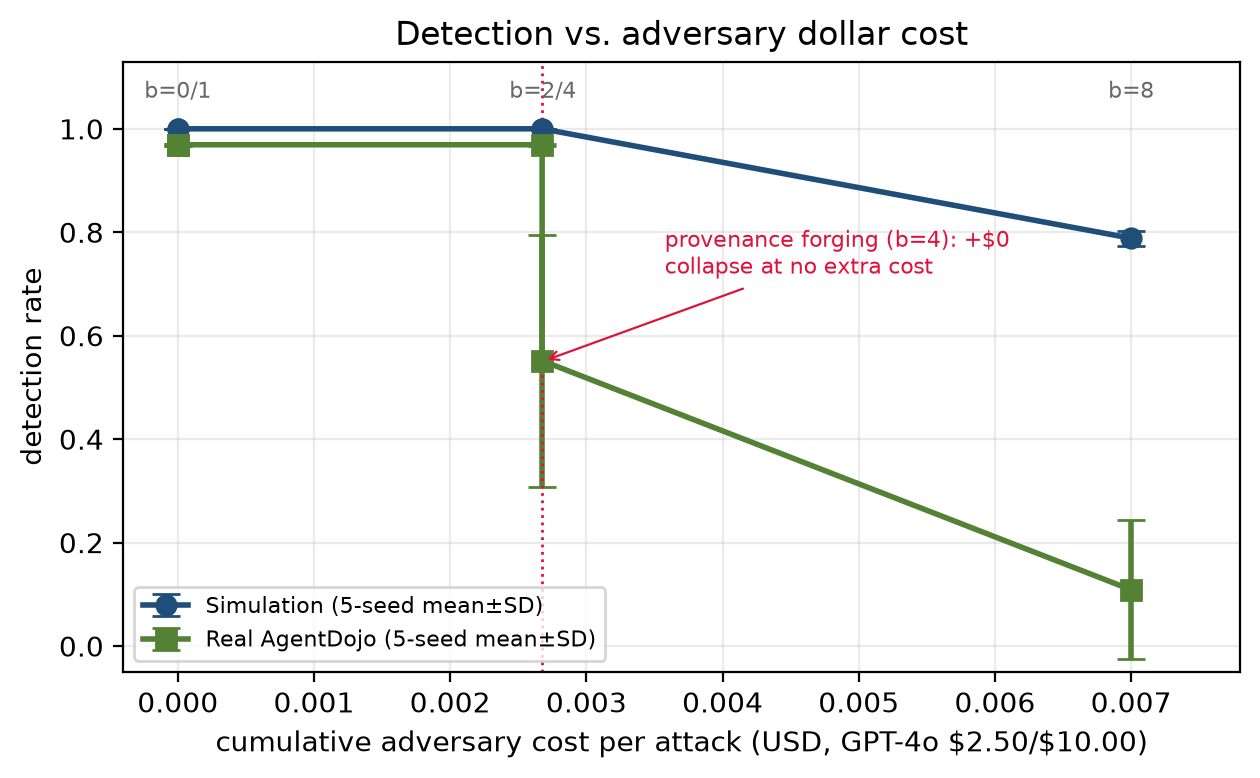
\includegraphics[width=\columnwidth]{figures/fig8_adaptive_dollars.png}
\caption{Detection versus cumulative adversary cost per attack (GPT-4o list pricing). Detection on real AgentDojo falls vertically at the provenance forging rung, which adds no dollar cost because it requires no model call; markers are labelled with the corresponding integer budget. Per rung token counts are order-of-magnitude estimates; the two zero-cost rungs are exact.}\label{fig:addollar}
\end{figure}

\section{Detectability: Coverage, Limits, and an Agenda}

The evaluation clarifies a distinction that the theory must now make precise where the difference between a signature existing and a detector being able to find it. Theorem 1 guarantees the former unconditionally. The latter cannot be guaranteed at all, and understanding exactly why is what turns the empirical contrast of the previous section into a principled research agenda rather than a list of disappointments. This section establishes the boundary between what is provable and what is not, maps the existing defense landscape against the signatures each defense approximates, and uses the boundary to organize the open problems.

Existence does not imply detectability for three distinct, compounding reasons. First, the benign behavior set $\mathcal{B}(u)$ is not given to any real detector, which must approximate it with an estimate $\hat{\mathcal{B}}(u)$ learned from a finite sample of benign runs; detection then tests whether a trajectory falls outside this estimate. A false positive occurs when a genuinely benign trajectory falls outside $\hat{\mathcal{B}}(u)$ because the sample failed to cover it; a false negative occurs when an attack trajectory falls inside the estimate because the estimate was too loose. The collapse observed in the AgentDojo evaluation follows from this reason, since no threshold can separate a poorly estimated benign set from the attacks.

Second, an adaptive adversary who knows the detector exists can select, among trajectories achieving the harmful effect, the one minimizing distance to the estimated benign set: a mimicry attack. This pushes the witnessing signature guaranteed by Theorem 1 arbitrarily close to the decision boundary; the theorem still holds, but its margin above the threshold can be driven to nothing, which is exactly what the fall to 0.79 in simulation and the sharper collapse on real data demonstrated empirically. This is the precise agent trajectory analogue of the mimicry attacks shown to defeat provenance graph host intrusion detectors \cite{r30}, and the host-security community's experience with that attack class is the best available warning here.

Third, the signatures require side information a deployment may lack: the first signature needs the allowed tool set, the fifth needs source and sink labels, and where such information is only partially available, the corresponding predicate becomes only partially decidable.

Together, these reasons establish that existence is provable, while detectability is empirical: a property of a particular detector against a particular distribution and adversary, measurable but never guaranteed by any theorem. Stating this boundary plainly is more useful than a guarantee that quietly assumes the estimated benign set equals the true one.Within this boundary, the existing defense landscape can be read as a collection of approximators, each targeting particular signatures, and organizing it this way reveals exactly where coverage runs out. A defense covers some subset of the six signatures, and Table~\ref{tab:approx} places the representative systems. Content- and model-level defenses sit upstream of the trajectory entirely and approximate none of the signatures directly \cite{r1}, \cite{r2}, \cite{r28}, which is the formal restatement of why they miss the cases that Theorem 1 locates in behavior: they are inspecting the wrong object. Execution-level defenses do better, approximating the first, second, and fifth signatures through task alignment checking and information flow control \cite{r13}, \cite{r15}, \cite{r16}. Trace- and graph based anomaly detectors approximate the fourth signature and, in their multi-agent forms, the sixth \cite{r14}, \cite{r19}, while probabilistic monitors estimate the reachability of unsafe states from partial trajectories \cite{r20}. The region left uncovered by the union of all these defenses, together with the cells that are nominally covered but only under side information that real deployments lack, is the formal target for new work: the set $\Phi_{\mathrm{gap}}$ of signatures that no current defense reliably approximates under realistic conditions.

\begin{table*}[t]\centering\caption{Existing defenses as approximators of behavioral signatures.}\label{tab:approx}\footnotesize\begin{tabular}{@{}p{4.2cm}p{2.6cm}p{8.4cm}@{}}\toprule
\textbf{Defense layer} & \textbf{Approx.} & \textbf{Key limitation} \\
\midrule
Content filters \cite{r1,r2} & none & benign looking payloads; adaptive bypass \cite{r5} \\
Instruction hierarchy \cite{r28} & none & static; fixed at training \\
Task alignment \cite{r13} & $\varphi_1$,$\varphi_2$ & needs clean task spec \\
Info-flow control \cite{r15,r16} & $\varphi_5$ & needs sink labels; utility cost \\
Trace/graph anomaly \cite{r14,r19} & $\varphi_4$,$\varphi_6$ & weak adaptive eval \cite{r30} \\
Probabilistic monitor \cite{r20} & $\varphi_4$ & coarse benign estimate \\
\bottomrule\end{tabular}\end{table*}

The boundary between Theorem 1 and the limits just described organizes the agenda directly, and the empirical results sharpen each item. The first and most important open problem is in-policy detection. The benchmarks show that the genuinely open challenge is not the out-of-policy attacks, which are caught almost trivially by the first and fifth signatures, but the in-policy reuse attacks, where the adversary accomplishes its goal entirely through tools the agent was already permitted to use, and the behavioral signal is correspondingly faint. Closing this gap, together with evaluating any proposed detector against the mimicry objective rather than against fixed attacks \cite{r5}, \cite{r30}, is the central challenge the field faces, and it is the one the results most directly motivate. The second open problem is the estimation of the benign behavior set itself: tighter, more sample-efficient, task conditioned models of benign behavior would directly shrink both error terms, and the AgentDojo result shows that this is currently the binding constraint in the hard regime. The third is a matter of benchmark infrastructure: the field lacks a shared corpus of benign and attacked agent trajectories at sufficient scale, and AgentDojo's small benign sample is a concrete instance of how that scarcity limits what can be measured. The fourth concerns composition: the sixth signature shows that compromise can propagate across agents, so the composition of detectors in multi-agent systems, where one agent's compromise becomes another agent's untrusted input, is an open and increasingly urgent problem as multi-agent deployments proliferate. Each of these is a concrete step from the existence guarantee that Theorem 1 provides toward the detectability that practice requires.

\section{Discussion}

The move from models that speak to agents that act relocates where security must be enforced. When a system only produces text, inspecting that text is a defensible strategy; once a system acts, risk moves to the actions, and inspecting text alone is structurally behind, since identical text can yield safe or catastrophic actions. The existence theorem makes this precise: behavioral evidence of a successful attack is guaranteed to exist, whereas content evidence is not. This asymmetry supports treating behavioral monitoring as the foundation of agent defense, not an optional supplement to content filtering.

Behavioral detection is solved in one regime and open in another. In the out-of-policy regime, where an attack must reach for a tool outside the agent's repertoire, detection is reliable. In the in-policy regime, where an attack hides among legitimate uses of legitimate tools, detection remains an open problem. A practitioner deploying a behavioral monitor should expect the former class of attacks to be caught reliably and the latter to be missed, and should architect accordingly. The most effective design lever is minimizing the privileges of an agent's in-policy tools, which shrinks the in-policy regime and pushes more attacks into the out-of-policy regime, where they are caught. An agent whose legitimate tools cannot themselves cause irreversible harm forces an attacker to introduce a new tool to do damage, and introducing a new tool is exactly what the strongest signatures detect. The value of least privilege for agents thus extends beyond the classical limiting of blast radius: it also converts hard-to-detect in-policy attacks into easier-to-detect out-of-policy ones.

\subsection{Least Privilege as Detectability Amplification}
In practice, an agent's access policy should be scoped to the specific user task, $\mathcal{T}_u\subset\mathcal{T}$, rather than defined globally for the entire system. Privileged actions, particularly those with irreversible external effects, should additionally require explicit justification, user confirmation, or trust elevation before execution.

The collapse of detection under mimicry, from near-perfect to well below half, is not a flaw specific to the detectors examined here but a property that any behavioral detector will exhibit against an adversary who optimizes to blend in; the theorem clarifies why, since the behavioral signature cannot be made to disappear but can be made arbitrarily hard to distinguish from noise. The implication is methodological: a behavioral defense that reports strong numbers only against fixed, nonadaptive attacks has not actually been tested on the threat that matters, and the field should treat adaptive evaluation as a requirement rather than an embellishment.


\subsection{Limitations}
The limitations bounding these claims are stated explicitly and gathered here. First, the formal model rests on the effect-through-action assumption, which holds for the tool calling agents studied here but would need re-examination for architectures in which an agent can affect the world through channels other than explicit tool calls. Second, the benign behavior set, treated by the theory as a well-defined semantic object, is in any real system only ever estimated, and the results show that the quality of that estimate is presently the binding constraint on detection in the hard regime. Third, the live benchmark evaluation exercises only one of the seven attack vectors, with the remaining six evaluated in simulation. Fourth, the in-policy analysis is conducted on AgentDojo trajectories reconstructed deterministically from the benchmark's ground truth annotations rather than collected from live agent runs; this fixes the denominators and isolates the provenance effect cleanly, but the reconstructed attacks carry the benchmark's canonical success and provenance labels by construction, so the provenance dependent detection figures ($0.968$ with $\varphi_5$, $0.151$ without) should be read as an ablation of the information flow signal under known labels rather than as a measurement of taint inferred by a deployed detector. Fifth, the strongest real-data detection result comes from InjecAgent, whose out-of-policy structure and benchmark-supplied sink labels make detection intrinsically easy, so that number bounds the favorable regime rather than the typical one. Finally, detection of in-policy compromise is load-bearing on provenance integrity: an adaptive adversary able to forge trust labels drives detection down at no model cost, which is a property of any provenance dependent detector and not specific to the signatures proposed here.

\section{Conclusion}

The shift from language models that speak to agents that act relocates security from the content an agent reads to the behavior it exhibits. A formal account is given of why this relocation is warranted and what it entails. A unified threat model places the field's incompatible adversary assumptions on a single set of five axes. Six behavioral signatures, defined as predicates over an agent's execution trajectory, make precise the observable ways in which a compromised agent departs from benign behavior. An existence theorem proves that any successful attack, whatever its injection vector, must produce at least one such departure in the agent's actions, paired, deliberately, with a precise account of why detecting that departure cannot be guaranteed against an adaptive adversary. An evaluation across two benchmarks and a controlled simulation maps exactly where behavioral detection works in practice: reliably when an attack must reach outside the agent's tool repertoire, and not yet when the attack reuses tools the agent already holds. The contribution is connective. A literature that has defined its adversary in ten different ways, and defended at whichever layer each paper happened to prefer, can now be read through a single question: which behavioral signature does this defense approximate, and how well does its estimate of benign behavior hold up against an adversary trying to stay inside it. The provable half of the answer is settled. The empirical half, and especially the detection of in-policy attacks under realistic benign data budgets, is where the work now lies.

\section*{Acknowledgment of AI Assistance}
The authors acknowledge the use of AI-based tools in the preparation of this work. Grammarly and Claude (Anthropic) were used to improve the grammar, clarity, and phrasing of the manuscript, and Claude was additionally used to assist in generating and refining portions of the supporting code. All code, experiments, and results were reviewed and verified by the authors, who take full responsibility for the content and conclusions of this paper.

\begin{thebibliography}{99}
\bibitem{r1} H. Inan et al., ``Llama Guard: LLM-based input-output safeguard for human-AI conversations,'' arXiv preprint arXiv:2312.06674, 2023.
\bibitem{r2} T. Rebedea, R. Dinu, M. N. Sreedhar, C. Parisien, and J. Cohen, ``NeMo Guardrails: A toolkit for controllable and safe LLM applications with programmable rails,'' in \emph{Proc. Conf. Empirical Methods Natural Lang. Process. (EMNLP): Syst. Demonstrations}, 2023, pp.~431--445, doi: 10.18653/v1/2023.emnlp-demo.40.
\bibitem{r3} X. Hou, Y. Zhao, S. Wang, and H. Wang, ``Model Context Protocol (MCP): Landscape, security threats, and future research directions,'' \emph{ACM Trans. Softw. Eng. Methodol.}, 2026, Art. no.~3796519, doi: 10.1145/3796519.
\bibitem{r4} OWASP Foundation, ``OWASP Top 10 for Large Language Model Applications,'' 2025. [Online]. Available: https://genai.owasp.org/
\bibitem{r5} M. Nasr, N. Carlini, C. Sitawarin, S. V. Schulhoff, J. Hayes, M. Ilie, J. Pluto, S. Song, H. Chaudhari, I. Shumailov, A. Thakurta, K. Y. Xiao, A. Terzis, and F. Tram`{e}r, ``The attacker moves second: Stronger adaptive attacks bypass defenses against LLM jailbreaks and prompt injections,'' arXiv preprint arXiv:2510.09023, 2025.
\bibitem{r6} Y. Shen, X. Pan, G. Hong, and M. Yang, ``Invisible threats from Model Context Protocol: Generating stealthy injection payload via tree-based adaptive search,'' arXiv preprint arXiv:2603.24203, 2026.
\bibitem{r7} Y. Liu, Y. Jia, R. Geng, J. Jia, and N. Z. Gong, ``Formalizing and benchmarking prompt injection attacks and defenses,'' in \emph{Proc. 33rd USENIX Security Symp.}, Philadelphia, PA, USA, Aug. 2024, pp.~1831--1847.
\bibitem{r8} E. Debenedetti, J. Zhang, M. Balunovi\'{c}, L. Beurer-Kellner, M. Fischer, and F. Tram\`{e}r, ``AgentDojo: A dynamic environment to evaluate prompt injection attacks and defenses for LLM agents,'' in \emph{Proc. Adv. Neural Inf. Process. Syst. (NeurIPS) Datasets Benchmarks Track}, 2024.
\bibitem{r9} Q. Zhan, Z. Liang, Z. Ying, and D. Kang, ``InjecAgent: Benchmarking indirect prompt injections in tool-integrated large language model agents,'' in \emph{Findings Assoc. Comput. Linguistics: ACL 2024}, Bangkok, Thailand, Aug. 2024, pp.~10471--10506, doi: 10.18653/v1/2024.findings-acl.624.
\bibitem{r10} H. Zhang, J. Huang, K. Mei, Y. Yao, Z. Wang, C. Zhan, H. Wang, and Y. Zhang, ``Agent Security Bench (ASB): Formalizing and benchmarking attacks and defenses in LLM-based agents,'' in \emph{Proc. Int. Conf. Learn. Represent. (ICLR)}, 2025.
\bibitem{r11} C. Huang, X. Huang, N. P. Tran, and A. Milani Fard, ``Model context protocol threat modeling and analysis of vulnerabilities to prompt injection with tool poisoning,'' \emph{J. Cybersecurity Privacy}, vol.~6, no.~3, Art. no.~84, 2026, doi: 10.3390/jcp6030084.
\bibitem{r12} J. T. Halloran, B. Radosevich, and G. Black, ``MCP safety audit: LLMs with the Model Context Protocol allow major security exploits,'' in \emph{Proc. SPIE, Assurance and Security for AI-Enabled Systems}, 2026, doi: 10.1117/12.3097390.
\bibitem{r13} F. Jia, T. Wu, X. Qin, and A. Squicciarini, ``The Task Shield: Enforcing task alignment to defend against indirect prompt injection in LLM agents,'' in \emph{Proc. 63rd Annu. Meeting Assoc. Comput. Linguistics (ACL): Long Papers}, 2025, pp.~29680--29697, doi: 10.18653/v1/2025.acl-long.1435.
\bibitem{r14} X. He, D. Wu, Y. Zhai, and K. Sun, ``SentinelAgent: Graph-based anomaly detection in multi-agent systems,'' arXiv preprint arXiv:2505.24201, 2025.
\bibitem{r15} F. Wu, E. Cecchetti, and C. Xiao, ``System-level defense against indirect prompt injection attacks: An information flow control perspective,'' arXiv preprint arXiv:2409.19091, 2024.
\bibitem{r16} P. Wang, Y. Liu, Y. Lu, Y. Cai, H. Chen, Q. Yang, J. Zhang, J. Hong, and Y. Wu, ``AgentArmor: Enforcing program analysis on agent runtime trace to defend against prompt injection,'' arXiv preprint arXiv:2508.01249, 2025.
\bibitem{r17} S. Rose, O. Borchert, S. Mitchell, and S. Connelly, ``Zero Trust Architecture,'' Nat. Inst. Standards Technol., Gaithersburg, MD, USA, Special Publication 800-207, Aug. 2020, doi: 10.6028/NIST.SP.800-207.
\bibitem{r18} S. Yan, L. Shi, W. Wang, J. Ren, Y. Li, and L. Sun, ``LLMBA: Efficient behavior analytics via large pretrained models in zero trust networks,'' \emph{IEEE Trans. Inf. Forensics Security}, vol.~21, pp.~2403--2415, 2026, doi: 10.1109/TIFS.2026.3666459.
\bibitem{r19} J. Liu, B. Ruan, X. Yang, Z. Lin, Y. Liu, Y. Wang, T. Wei, and Z. Liang, ``TraceAegis: Securing LLM-based agents via hierarchical and behavioral anomaly detection,'' arXiv preprint arXiv:2510.11203, 2025.
\bibitem{r20} H. Wang, C. M. Poskitt, J. Wei, and J. Sun, ``ProbGuard: Probabilistic runtime monitoring for LLM agent safety,'' arXiv preprint arXiv:2508.00500, 2025.
\bibitem{r21} F. Maggi, M. Matteucci, and S. Zanero, ``Detecting intrusions through system call sequence and argument analysis,'' \emph{IEEE Trans. Dependable Secure Comput.}, vol.~7, no.~4, pp.~381--395, Oct.--Dec. 2010, doi: 10.1109/TDSC.2008.69.
\bibitem{r22} M. Villarreal-Vasquez, G. Modelo-Howard, S. Dube, and B. Bhargava, ``Hunting for insider threats using LSTM-based anomaly detection,'' \emph{IEEE Trans. Dependable Secure Comput.}, vol.~20, no.~1, pp.~451--462, Jan./Feb. 2023, doi: 10.1109/TDSC.2021.3135639.
\bibitem{r23} C. Xiong, T. Zhu, W. Dong, L. Ruan, R. Yang, Y. Cheng, Y. Chen, S. Cheng, and X. Chen, ``CONAN: A practical real-time APT detection system with high accuracy and efficiency,'' \emph{IEEE Trans. Dependable Secure Comput.}, vol.~19, no.~1, pp.~551--565, 2022, doi: 10.1109/TDSC.2020.2971484.
\bibitem{r24} L. Cheng, K. Tian, D. D. Yao, L. Sha, and R. A. Beyah, ``Checking is believing: Event-aware program anomaly detection in cyber-physical systems,'' \emph{IEEE Trans. Dependable Secure Comput.}, vol.~18, no.~2, pp.~825--842, 2021, doi: 10.1109/TDSC.2019.2906161.
\bibitem{r25} F. He, T. Zhu, D. Ye, B. Liu, W. Zhou, and P. S. Yu, ``The emerged security and privacy of LLM agent: A survey with case studies,'' \emph{ACM Comput. Surv.}, vol.~58, no.~6, 2025, doi: 10.1145/3773080.
\bibitem{r26} A. Chhabra, S. Datta, S. K. Nahin, and P. Mohapatra, ``Agentic AI security: Threats, defenses, evaluation, and open challenges,'' \emph{IEEE Access}, vol.~14, pp.~49455--49482, 2026, doi: 10.1109/ACCESS.2026.3675554.
\bibitem{r27} K. C. Roy and G. Chen, ``GraphCH: A deep framework for assessing cyber-human aspects in insider threat detection,'' \emph{IEEE Trans. Dependable Secure Comput.}, vol.~21, no.~5, pp.~4495--4509, 2024, doi: 10.1109/TDSC.2024.3353929.
\bibitem{r28} E. Wallace, K. Xiao, R. Leike, L. Weng, J. Heidecke, and A. Beutel, ``The instruction hierarchy: Training LLMs to prioritize privileged instructions,'' arXiv preprint arXiv:2404.13208, 2024.
\bibitem{r29} W. Yang, X. Bi, Y. Lin, S. Chen, J. Zhou, and X. Sun, ``Watch out for your agents! Investigating backdoor threats to LLM-based agents,'' in \emph{Proc. Adv. Neural Inf. Process. Syst. (NeurIPS)}, 2024.
\bibitem{r30} A. Goyal, X. Han, G. Wang, and A. Bates, ``Sometimes, you aren't what you do: Mimicry attacks against provenance graph host intrusion detection systems,'' in \emph{Proc. Netw. Distrib. Syst. Secur. Symp. (NDSS)}, 2023, doi: 10.14722/ndss.2023.24207.
\bibitem{r31} X. Bouthillier et al., ``Accounting for variance in machine learning benchmarks,'' in \emph{Proc. Mach. Learn. Syst. (MLSys)}, vol.~3, 2021, pp.~747--769.
\end{thebibliography}

\end{document}